\documentclass[9pt,twocolumn]{scrartcl}

%\documentclass[9pt]{sigcomm-alternate}

%\usepackage[margin=1in,bottom=1.2in]{geometry}
\usepackage{amsfonts,amssymb,amsmath}
\usepackage[thmmarks,hyperref,amsthm,amsmath]{ntheorem}
\usepackage{graphicx}
\usepackage[ruled,vlined,commentsnumbered]{algorithm2e}
\usepackage[usenames,dvipsnames]{color}
\usepackage{hyperref}
\usepackage{multirow}
\usepackage{lineno}
\usepackage[shortlabels]{enumitem}
\usepackage[utf8]{inputenc}
\usepackage[OT4]{fontenc}
\usepackage{comment}
\usepackage{fancyhdr}
\usepackage{tikz}
%Used Symbols
%c_i = chunk i
%v_i = vm i
%b_t = transfer bandwidth
%b_c = pairwise communication bandwidth
%n = |VMs| = |Chunks|


%Header Extensions Seperation
%Carlo
\newcommand{\VmSlot}{\text{VM slot}}
\newcommand{\VmSlots}{\VmSlot\text{s}}
\newcommand{\Capacity}{\ensuremath{\textsc{cap}}}
\newcommand{\VM}{\textsc{VM}}
\newcommand{\Problem}{\textsc{DummyName Problem}}
\newcommand{\carlo}[1]{\textcolor{red}{#1}}
\newcommand{\maciek}[1]{\textcolor{green}{#1}}
\newcommand{\MaFactor}{\ensuremath{\textsc{MA}}}
\newcommand{\Path}{\ensuremath{p}}
\newcommand{\RedundancyFactor}{\ensuremath{r}}

\newcommand{\VmChunkAssignment}{\ensuremath{ASS_v}}
\newcommand{\NodeMapping}{\ensuremath{MAP_v}}
\newcommand{\ChunkLocation}{\ensuremath{\textsc{loc}}}

\newcommand{\ChunkType}{\ensuremath{textsc{ct}}}
\newcommand{\VirtualNodes}{\ensuremath{V_V}}
\newcommand{\VirtualEdges}{\ensuremath{E_V}}
\newcommand{\VirtualNode}{\ensuremath{v}}
\newcommand{\VirtualEdge}{\ensuremath{e}}
\newcommand{\VCSwitch}{\ensuremath{\textsc{center}}}
\newcommand{\SubstrateNodes}{\ensuremath{V_S}}
\newcommand{\SubstrateEdges}{\ensuremath{E_S}}
\newcommand{\SubstrateNode}{\ensuremath{v}}
\newcommand{\SubstrateEdge}{\ensuremath{e}}
\newcommand{\Leaf}{\ensuremath{l}}
\newcommand{\Leaves}{\ensuremath{L}}
\newcommand{\Chunks}{\ensuremath{\textsc{chunks}}}
\newcommand{\aroot}{\emph{root}}

\newcommand{\clauses}{\alpha}
\newcommand{\vars}{\beta}
\newcommand{\variables}{\beta}
\newcommand{\achunk}{\ensuremath{c}}
\newcommand{\Chunk}{\ensuremath{c}}
\newcommand{\capa}{\emph{cap}}
\newcommand{\capacity}{\emph{cap}}
\newcommand{\Distance}{\emph{\textsc{dist}}}
\newcommand{\dist}{\emph{dist}}
\newcommand{\CostPerChunk}{\emph{cost}}


\newcommand{\VC}{\textsc{VC}}
\newcommand{\CC}{\textsc{NI}}

\newcommand{\VE}{\textsc{VE}}
\newcommand{\FP}{\textsc{FP}}
\newcommand{\RS}{\textsc{RS}}
\newcommand{\BW}{\textsc{BW}}
\newcommand{\MA}{\textsc{MA}}
\newcommand{\Cost}{\textsc{F}}

\newcommand{\MatchCost}{\textsc{MCost}}
\newcommand{\chunkOf}{\textsc{chunkOf}}


%Maciek

\newcommand{\Bandwidth}{\ensuremath{bw}}
\newcommand{\Tree}{\ensuremath{T}}
\newcommand{\CostCom}{\ensuremath{b_1}}
\newcommand{\CostTrans}{\ensuremath{b_2}}
\newcommand{\Vms}{\ensuremath{n}}
\newcommand{\TSC}{\textsc{3-SC}}
\newcommand{\TDM}{\textsc{3-DM}}
\newcommand{\TSAT}{\textsc{3-Sat}}
\newcommand{\NSAT}{\textsc{Sat}}
\newcommand{\SAT}{\textsc{Sat}}
\newcommand{\ZSAT}{\textsc{2-Sat}}


\newcommand{\Formula}{\ensuremath{\Psi}}
\newcommand{\Clauses}{\ensuremath{Cl(\Formula)}}
\newcommand{\NClauses}{\ensuremath{c}}
\newcommand{\Vars}{\ensuremath{Var(\Formula)}}
\newcommand{\NVars}{\ensuremath{|\Vars|}}
\newcommand{\ChunkTypes}{\ensuremath{ch}}
\newcommand{\Thr}{\ensuremath{Th}}
\newcommand{\VCB}{\ensuremath{VCB}}
\newcommand{\VCNB}{\ensuremath{VCNB}}
\newcommand{\varx}{\ensuremath{x}}
\newcommand{\positive}{\ensuremath{positive}}
\newcommand{\negative}{\ensuremath{negative}}
\newcommand{\Val}{\ensuremath{Val}}
\newcommand{\Sol}{\ensuremath{SOL}}



\definecolor{blueLink}{rgb}{0,0.2,0.8}
\hypersetup{colorlinks,linkcolor=blueLink,urlcolor=blueLink,citecolor=blueLink}
\newcommand{\lref}[2][]{\hyperref[#2]{#1~\ref*{#2}}}



%%%%%%%%%%%%%%%%%%%%%%%%%%%%%%%%%%%%%%%%%%%%%%%%%%%%%%%%%%%%%
% GENERAL STYLE MACROS
%%%%%%%%%%%%%%%%%%%%%%%%%%%%%%%%%%%%%%%%%%%%%%%%%%%%%%%%%%%%%

\newcommand{\etal}{{\it et~al.\ }}
\newcommand{\myparagraph}[1]{{\smallskip\noindent{\bf #1}}}
\newcommand{\mycase}[1]{{\underline{Case~#1}:}}

%%%%%%%%%%%%%%%%%%%%%%%%%%%%%%%%%%%%%%%%%%%%%%%%%%%%%%%%%%%%
% THEOREMS AND SUCH
%%%%%%%%%%%%%%%%%%%%%%%%%%%%%%%%%%%%%%%%%%%%%%%%%%%%%%%%%%%%%

\newtheorem{theorem}{Theorem}
\newtheorem{corollary}[theorem]{Corollary}
\newtheorem{lemma}[theorem]{Lemma}
\newtheorem{claim}[theorem]{Claim}
\newtheorem{fact}{Fact}

%%%%%%%%%%%%%%%%%%%%%%%%%%%%%%%%%%%%%%%%%%%%%%%%%%%%%%%%%%%%%
% USEFUL LETTERS
%%%%%%%%%%%%%%%%%%%%%%%%%%%%%%%%%%%%%%%%%%%%%%%%%%%%%%%%%%%%%

\DeclareMathOperator{\polylog}{polylog}
\newcommand{\emdash}{\hspace{1mm}---\hspace{1mm}}
\newcommand{\e}{\mathrm{e}}
\renewcommand{\O}{\mathcal{O}}
\renewcommand{\Pr}{\mathbf{Pr}}
\newcommand{\E}{\mathbf{E}}
\newcommand{\NAT}{\mathbb{N}}
\newcommand{\REAL}{\mathbb{R}}

%%%%%%%%%%%%%%%%%%%%%%%%%%%%%%%%%%%%%%%%%%%%%%%%%%%%%%%%%%%%%
% PARENTHESES ETC
%%%%%%%%%%%%%%%%%%%%%%%%%%%%%%%%%%%%%%%%%%%%%%%%%%%%%%%%%%%%%

\newcommand{\ceiling}[1]{\left\lceil #1 \right\rceil}
\newcommand{\floor}[1]{\left\lfloor #1 \right\rfloor}
\newcommand{\braced}[1]{{\left\{#1\right\}}}
\newcommand{\bigbrackd}[1]{{\big[#1\big]}}
\newcommand{\brackd}[1]{{\left[#1\right]}}
\newcommand{\parend}[1]{{\left(#1\right)}}

%%%%%%%%%%%%%%%%%%%%%%%%%%%%%%%%%%%%%%%%%%%%%%%%%%%%%%%%%%%%%
% FRACTIONS
%%%%%%%%%%%%%%%%%%%%%%%%%%%%%%%%%%%%%%%%%%%%%%%%%%%%%%%%%%%%%

\newcommand{\half}{\frac{1}{2}}
\newcommand{\onehalf}{\frac{1}{2}}
\newcommand{\onethird}{\frac{1}{3}}
\newcommand{\twothirds}{{\textstyle\frac{2}{3}}}
\newcommand{\fourthirds}{{\textstyle\frac{4}{3}}}
\newcommand{\fivethirds}{{\textstyle\frac{5}{3}}}
\newcommand{\threefourths}{{\textstyle\frac{3}{4}}}

%%%%%%%%%%%%%%%%%%%%%%%%%%%%%%%%%%%%%%%%%%%%%%%%%%%%%%%%%%%%%
% ALGORITHM NAMES, ETC
%%%%%%%%%%%%%%%%%%%%%%%%%%%%%%%%%%%%%%%%%%%%%%%%%%%%%%%%%%%%%

\newcommand{\ALG}{\textsc{Alg}}
\newcommand{\OPT}{\textsc{Opt}}
\newcommand{\DET}{\textsc{Det}}
\newcommand{\RAND}{\textsc{Rand}}

%%%%%%%%%%%%%%%%%%%%%%%%%%%%%%%%%%%%%%%%%%%%%%%%%%%%%%%%%%%%%
% PSEUDOCODE
%%%%%%%%%%%%%%%%%%%%%%%%%%%%%%%%%%%%%%%%%%%%%%%%%%%%%%%%%%%%%

\newcommand{\IF}    {{\bf if }}
\newcommand{\THEN}  {{\bf then }} 
\newcommand{\FOR}   {{\bf for }}
\newcommand{\EACH}  {{\bf each }} 
\newcommand{\DO}  {{\bf do }} 

%%%%%%%%%%%%%%%%%%%%%%%%%%%%%%%%%%%%%%%%%%%%%%%%%%%%%%%%%%%%%
% EDITORIAL MACROS
%%%%%%%%%%%%%%%%%%%%%%%%%%%%%%%%%%%%%%%%%%%%%%%%%%%%%%%%%%%%%

\definecolor{brown}{rgb}{0.4,0,0} 
\definecolor{purple}{rgb}{0.2,0,0.6}
\definecolor{hotpink}{rgb}{1,0.4,0.7}
\newcommand{\marginnote}[1]{\marginpar{\scriptsize{\begin{flushleft}#1\end{flushleft}}}}
\newcommand{\todo}[1]{\noindent\colorbox{red}{todo: #1}} 
\newcommand{\marcin}[1]{\color{red} Marcin: #1\color{black}}



\title{A Note on Virtual Cluster Embedding with Data Locality}

\title{Embedding Algorithms for Virtual Clusters with Data Locality and Replica Selection}

\title{Embedding Virtual Clusters with Data Locality and Replica Selection\\{\Large Real Algorithms for Virtual Environments}}

\title{Data Locality and Replica Aware Virtual Cluster Embeddings for Fat-Trees}
%\\{\Large Real Algorithms for Virtual Environments}}


\author{Carlo Fuerst$^1$, Maciek Pacut$^2$, Stefan Schmid$^3$\\
$^1$ TU Berlin, Germany; $^2$ University of Wroclaw, Poland; $^3$ TU Berlin \& T-Labs, Germany}

\begin{document}

\maketitle


\begin{abstract}
\textbf{Abstract.} Virtualized datacenters offer great flexibilities in terms of resource allocation. In particular, by
decoupling applications from the constraints of the underlying physical infrastructure, virtualization
supports an optimized mapping of virtual machines as well as their interconnecting network (the so-called \emph{virtual cluster}) to their
physical counterparts: essentially a graph embedding problem.

However, existing algorithms
in the literature often ignore a crucial dimension of the embedding problem, namely \emph{data locality}:
the input to a cloud application such as MapReduce is typically stored in a distributed,
and sometimes redundant, file system or database. Since moving this data is costly, an embedding algorithm should be data locality aware,
and allocate computation close to the data; in case of redundant storage, the algorithm should also optimize the \emph{replica selection}.

This paper initiates the algorithmic study of data locality aware virtual cluster embeddings in fat-tree like datacenter topologies.
In particular, we
show that
despite the many degrees of freedom of the embedding, many problems can be
solved efficiently, and we highlight interesting connections
to classic optimization problems, such as matchings
flow problems. However, we also show the limitations of such optimizations,
by presenting several new NP-hardness results; interestingly,
our hardness proofs are for uncapacitated settings.
\end{abstract}

%%%%%%%%%%%%%%%%%%%%%%%%%%%%%%%%%%%%%
\section{Introduction}

Server virtualization has revamped the server business over the last years,
and has radically changed the way we think about resource allocation:
today, almost arbitrary computational resources can be allocated on demand.
Moreover, the virtualization trend now started to spill over to the network:
batch-processing applications such as MapReduce often generate significant
network traffic (namely during the so-called shuffle phase)~\cite{amazonbw},
and in order to avoid interference in the underlying physical network and in order to provide a predictable
application performance, it is important to provide performance isolation and bandwidth guarantees
for the virtual network connecting the virtual machines.~\cite{talk-about}

Server and network virtualization introduces interesting resource allocation flexibilities,
in the sense that virtual machines and their interconnecting network,
can in principle be embedded \emph{anywhere} in the datacenter. The resulting flexibilities
can be exploited for various optimizations;
however, the joint optimization of node and link mapping is often non-trivial.~\cite{pb-embed}
Over the last years, especially the problem of embedding
\emph{Virtual Clusters} has been studied intensively. Virtual clusters are the most popular abstraction for batch-processing applications:
a virtual cluster connects a set of virtual machines by providing pair-wise bandwidth guarantees.
In order to provide resource-efficiency, existing algorithms aim to map virtual machines as close as possible
in the datacenter, which minimizes communication costs.~\cite{oktopus,proteus}

However, existing embedding algorithms often ignore an important aspect: the fact that the input data
to batch-processing applications,
the so-called \emph{chunks}, are stored in a distributed file system or database. In order to minimize
costly data transmissions, an embedding algorithm should be \emph{data locality aware},
and map compute units close to the chunk locations. Moreover, in case of redundant storage (batch processing
applications often provide a 3-fold redundancy), the algorithm should exploit flexibilities in
the \emph{(chunk) replica selection}.

\subsection{Our Contributions}

This paper initiates the study of data-locality and replica aware embedding problems in virtualized datacenters.
In particular, we decompose the optimization problem into different fundamental models, in terms of flexible
node placement, capacity constraints, or replication,
and draw an almost complete picture of the problem space. Concretely, we show that several problems
can be solved optimally in polynomial time, despite the large degrees of freedom, and also highlight
computational hardness limitations. Interestingly, while it is well-known that (unsplittable) multi-commodity flow
problems are NP-hard in capacitated networks, our results highlight the hardness of several uncapacitated
optimization problems. In particular, we show that NP-hard problems already arise in trees of height two,
and even if the number of replicas is bounded by two.


\subsection{Organization}

The remainder of this paper is organized as follows.
Section~\ref{sec:model} introduces our formal model in detail.
Algorithms are presented in Section~\ref{sec:poly} and
hardness results are presented in Section~\ref{sec:np}.
After discussing related work in Section~\ref{sec:relwork},
we conclude our work in Section~\ref{sec:conclusion}.


\section{Model}\label{sec:model}

We will first present our model formally, and subsequently discuss how it relates
to batch-processing applications.

\textbf{Fundamental Parts.} Our model consists of three fundamental parts: (1) the substrate network,
(2) the input data, and
(3) the virtual network.

The substrate network (also known as the \emph{host graph}) describes the physical resources:
a set $S$ of $n_S=|S|$ servers interconnected by a network. Concretely, we assume
that the servers are interconnected by a tree network, using a set $R$ of routers and a set $E$ of links,
where the servers are located at the tree leaves. Each server $s\in S$ has a certain number
$\capacity(s)$ of available slots for hosting virtual machines, and each link $e\in E$ has a certain bandwidth
capacity $\capacity(e)$.

The problem input is stored in the form of \emph{chunk types} $\{\achunk_1, \ldots, \achunk_k\}$.  For each chunk type $\achunk_i$,
there exist $r$ replicas $\{\achunk_{i,1},\ldots, \achunk_{i,r}\}$, where each replica is stored at a certain server.
Concretely, for each of the $r\cdot k$ replicas $\achunk_{i,j}$, we will denote by $\pi(\achunk_{i,j})$ at
which server it is stored. Only one replica is chosen for processing, and we will refer to this
replica as the \emph{active} (or selected) replica.

The virtual network consists of a set $\VirtualNodes$ of $n_v=|\VirtualNodes|$ virtual machines (henceforth often simply called \emph{nodes}).
Each node $v$ can be placed (or, synonymously, \emph{embedded}) on a server; if the capacity $\capacity(s)$ of server $s$ is sufficiently high, multiple nodes can be hosted on $s$. We will denote the server of node $v$ by $\pi(v)$.
Since these virtual machines process the input data, they need to be assigned and connected to the
chunks. Concretely, for each chunk type $\achunk_i$, one replica $\achunk_{i,j}$ must be processed by exactly one virtual machine $v$;
which replica $\achunk_{i,k}$ is chosen is subject to optimization.
We will denote by $\mu$ the matching of virtual machines to chunks; a virtual machine
may have to process multiple chunks, but the number of chunks per node must be constant.
In order to provide performance guarantees, both the connection to the chunks
as well as the interconnection between the virtual machines must provide a certain
minimal bandwidth guarantee; we will refer to the first type of network as the \emph{access
network}, and to the second type of network as the \emph{inter-connect}. The inter-connect will
is modelled as a complete network (a virtual cluster). Concretely, we assume that an  active chunk
is connected to its node at a minimal bandwidth $\CostTrans$, and a node is connected to any other node
at minimal bandwidth $\CostCom$.

\textbf{Optimization Objective.} Our goal is to develop algorithms which minimize
the resource footprint: the overall bandwidth allocation in the datacenter. That is,
we aim to embed the virtual machines in a locality-aware manner, close to the input data
(the chunks), as well as close to
each other. Let $\dist(v,\achunk)$ denote the distance (in the underlying physical network $\Tree$) between a node $v$ and a
chunk $\achunk$, and let $\dist(v_1,v_2)$ denote the distance between the two nodes $v_1$ and $v_2$.
We define the footprint $\Cost(v)$ of a node $v$ as follows:
$$
\Cost(v) = \sum_{\achunk\in C(v)} \CostTrans \cdot \dist(v,\achunk) + \sum_{v' \in \VirtualNodes\setminus\{v\}} \CostCom \cdot d(v,v'),
$$
where $C(v)$ is the set of chunks assigned to $v$. Our goal is to minimize the overall footprint
$\Cost=\sum_v \Cost(v)$.


FIXME: add an overview picture

\textbf{Problem Decomposition.}
In order to provide a complete picture of the tractability and intractability of different
problem variants, we decompose our problem into its fundamental aspects.

\emph{Replica Selection $\RS$.} The first fundamental problem is replica selection: 
if the input data is stored redundantly, the algorithm needs to choose a replica
for each chunk type, and assign it to a virtual machine. We will refer to a scenario
where there are redundant chunks and a replica needs to be selected by $\RS$. Note that this
selection or ``matching problem'' is non-trivial, even if the locations of the virtual machines
are already given. 

\emph{Multiple Assignment $\MA$.} Sometimes, we will assume that each virtual machine
needs to process at most one chunk, and we will refer to the problem variant where there are multiple chunks to process per virtual 
machine by $\MA$. 

\emph{Flexible Placement $\FP$.} We will refer to a scenario where also the location of the virtual machines is subject to optimization,
by $\FP$.

\emph{Node Interconnect $\CC$.} We will distinguish between scenarios where inter-connects between virtual machines (with $\CostCom>0$) are needed,
 and scenarios where only the access to the replicas requires bandwidth reservations. We will refer to scenarios
  with interconnects by $\CC$. 

\emph{Bandwidth Capacities $\BW$.} We distinguish between an uncapacitated and a capacitated scenario where the links 
of the substrate network come with bandwidth
constraints, and will refer to the bandwidth-constrained version by $\BW$; the capacity of servers
(the number of virtual machines which can be hosted concurrently) is always limited.


\textbf{Remark on Practical Motivation.}
Our model is inspired by batch-processing applications such as MapReduce.
The standard datacenter topology today are fat-trees~\cite{fattree},
and the most popular virtual network abstraction is the virtual cluster~\cite{oktopus}.
MapReduce applications cycle through three main phases: during the first phase,
the input data is mapped in a distributed fashion, by the mappers.
The resulting output is then transmitted to the so-called reducers; this phase is
called the shuffling phase. In the third phase, the data is processed by the reducers.
Moreover, in the beginning resp.~in the end, data needs to be loaded from resp.~written
back to the distributed file system.
Typically, a node serves both as a mapper and a reducer.

In our formal model, we distinguish between the bandwidth $\CostTrans$ needed to
transmit the input data to its assigned node, and the bandwidth $\CostCom$
needed during the shuffling phase between the virtual nodes.
The ratio $\CostCom/\CostTrans$ can be seen as the so-called mapping ratio:
how much smaller is the input after the mapping phase.


%%%%%%%%%%%%%%%%%%%%%%%%%%%%%%%%%%%%%
\section{Polynomial-Time Algorithms}\label{sec:poly}

Our data locality and replica aware virtual cluster embeddings
problem exhibits interesting connections to classic matching and
flow problems. In this section, we point out these connections and
exploit them to devise polynomial-time algorithms for a wide range
of problem variants. We also show that a large number of problems
can be solved optimally using dynamic programming. Note that all proposed
algorithms solve the problem optimally w.r.t. to the overall bandwidth costs
independently of $\CostTrans$ and (if present in the properties) $\CostCom$ and
$\Capacity$

\subsection{Matching based solutions}

Some versions of $\Problem$ boil down to matching problems. These are in
particular problems related to replica seletion, e.g. the basic version of
$\Problem$: each VM
is allready placed, the loactions of all chunks are known, and we have to
compute an assignment (or matching) of VMs to chunks, such that each VM is
assigned to
exactly one chunk, and each chunk is assigned to exactly one chunk. Hence we
can transform each instance of the basic $\Problem$ to a minimum weight
perfect bipartite
matching problem\cite{schrijver_combinatorial_optimization}. One of the sets
is formed by $\VirtualNodes$, the other by the
set of chunks. A VM has an edge to each chunk. The costs of these edges are
defined by the hop count between the VM and the chunk in the host graph. Each
edge which is chosen for the solution of the matching problem, indicates that
the chunk is assigned to the vm of the edge.

\begin{figure}
\begin{minipage}[b]{0.49\linewidth}
\centering
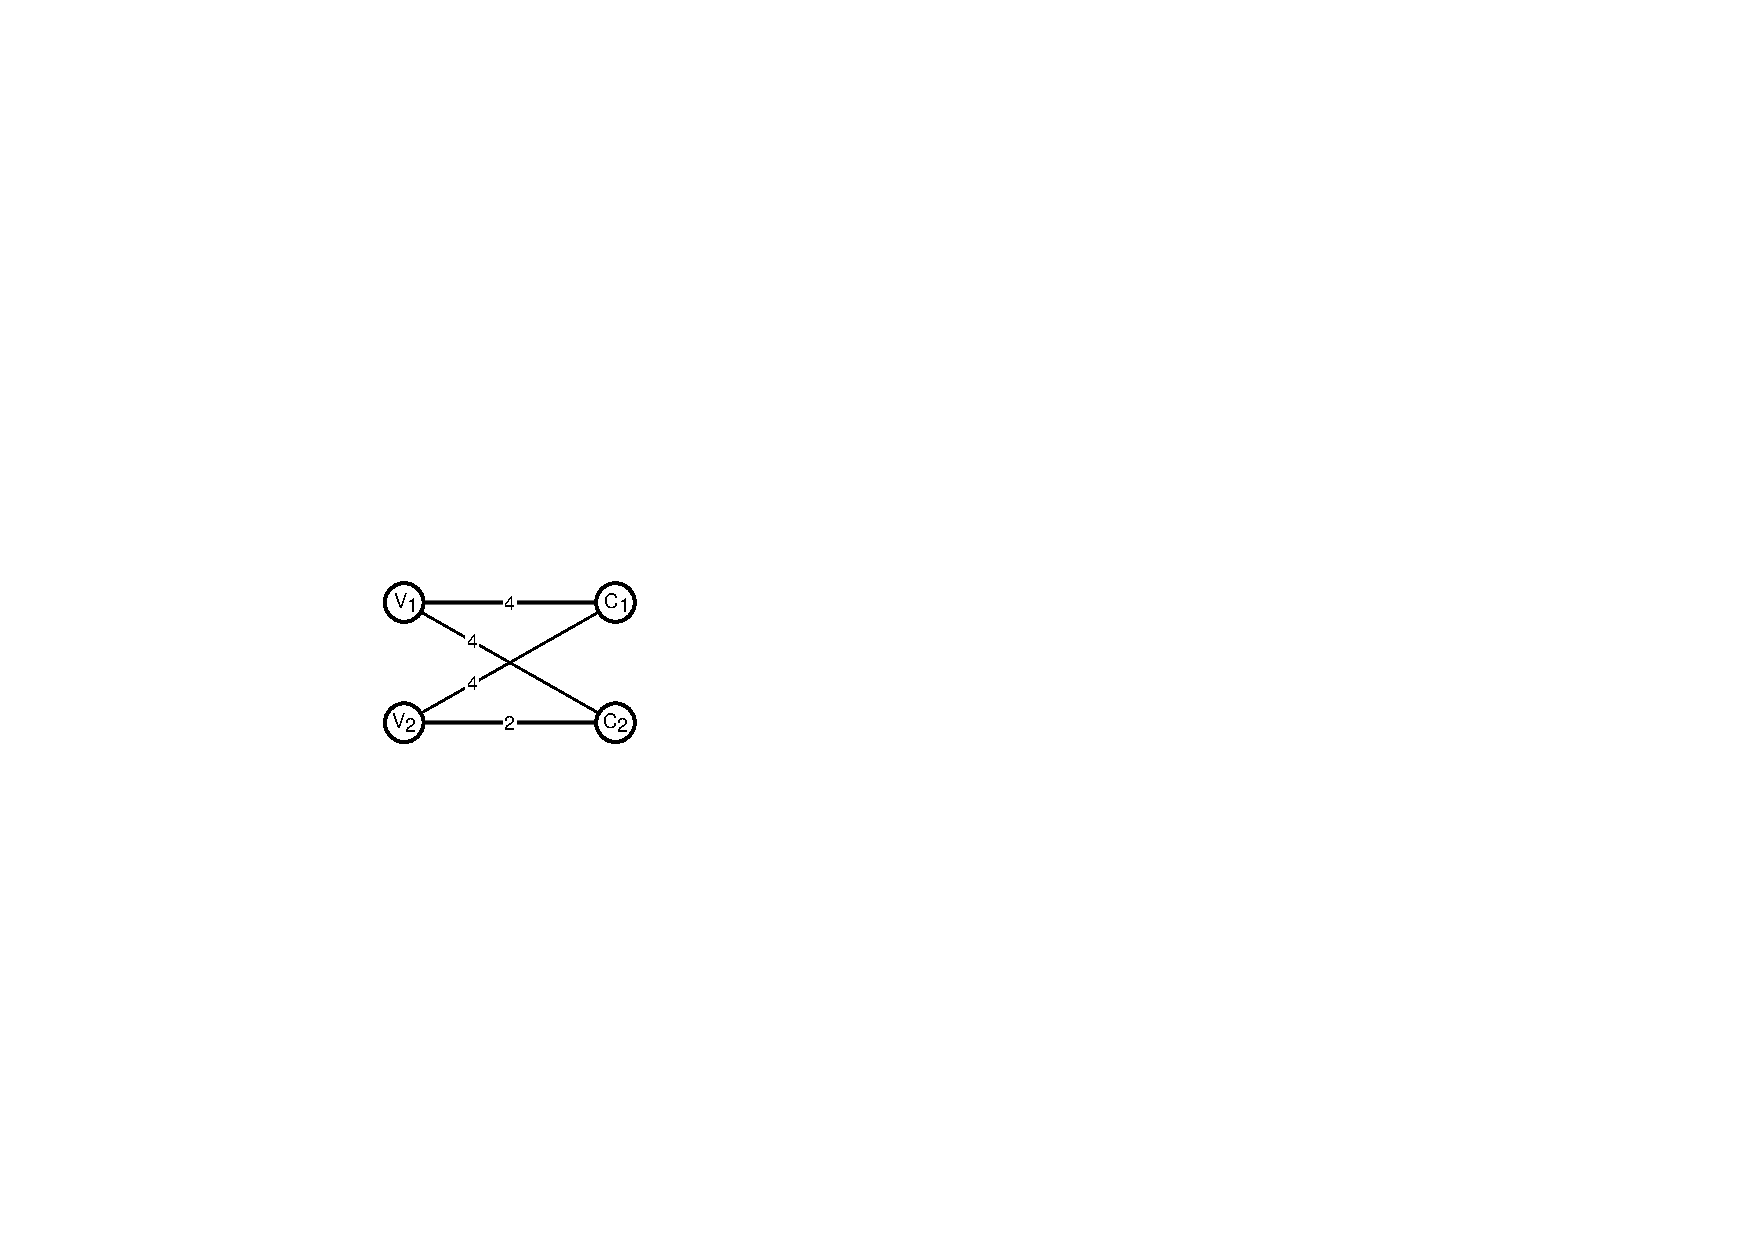
\includegraphics[width =\columnwidth]{figs/matching_basic}
\caption{The matching problem generated from the basic scenario in
Figure~\ref{fig:basic_problem}}
\label{fig:matching_basic}
\end{minipage}
\quad
\begin{minipage}[b]{0.49\linewidth}
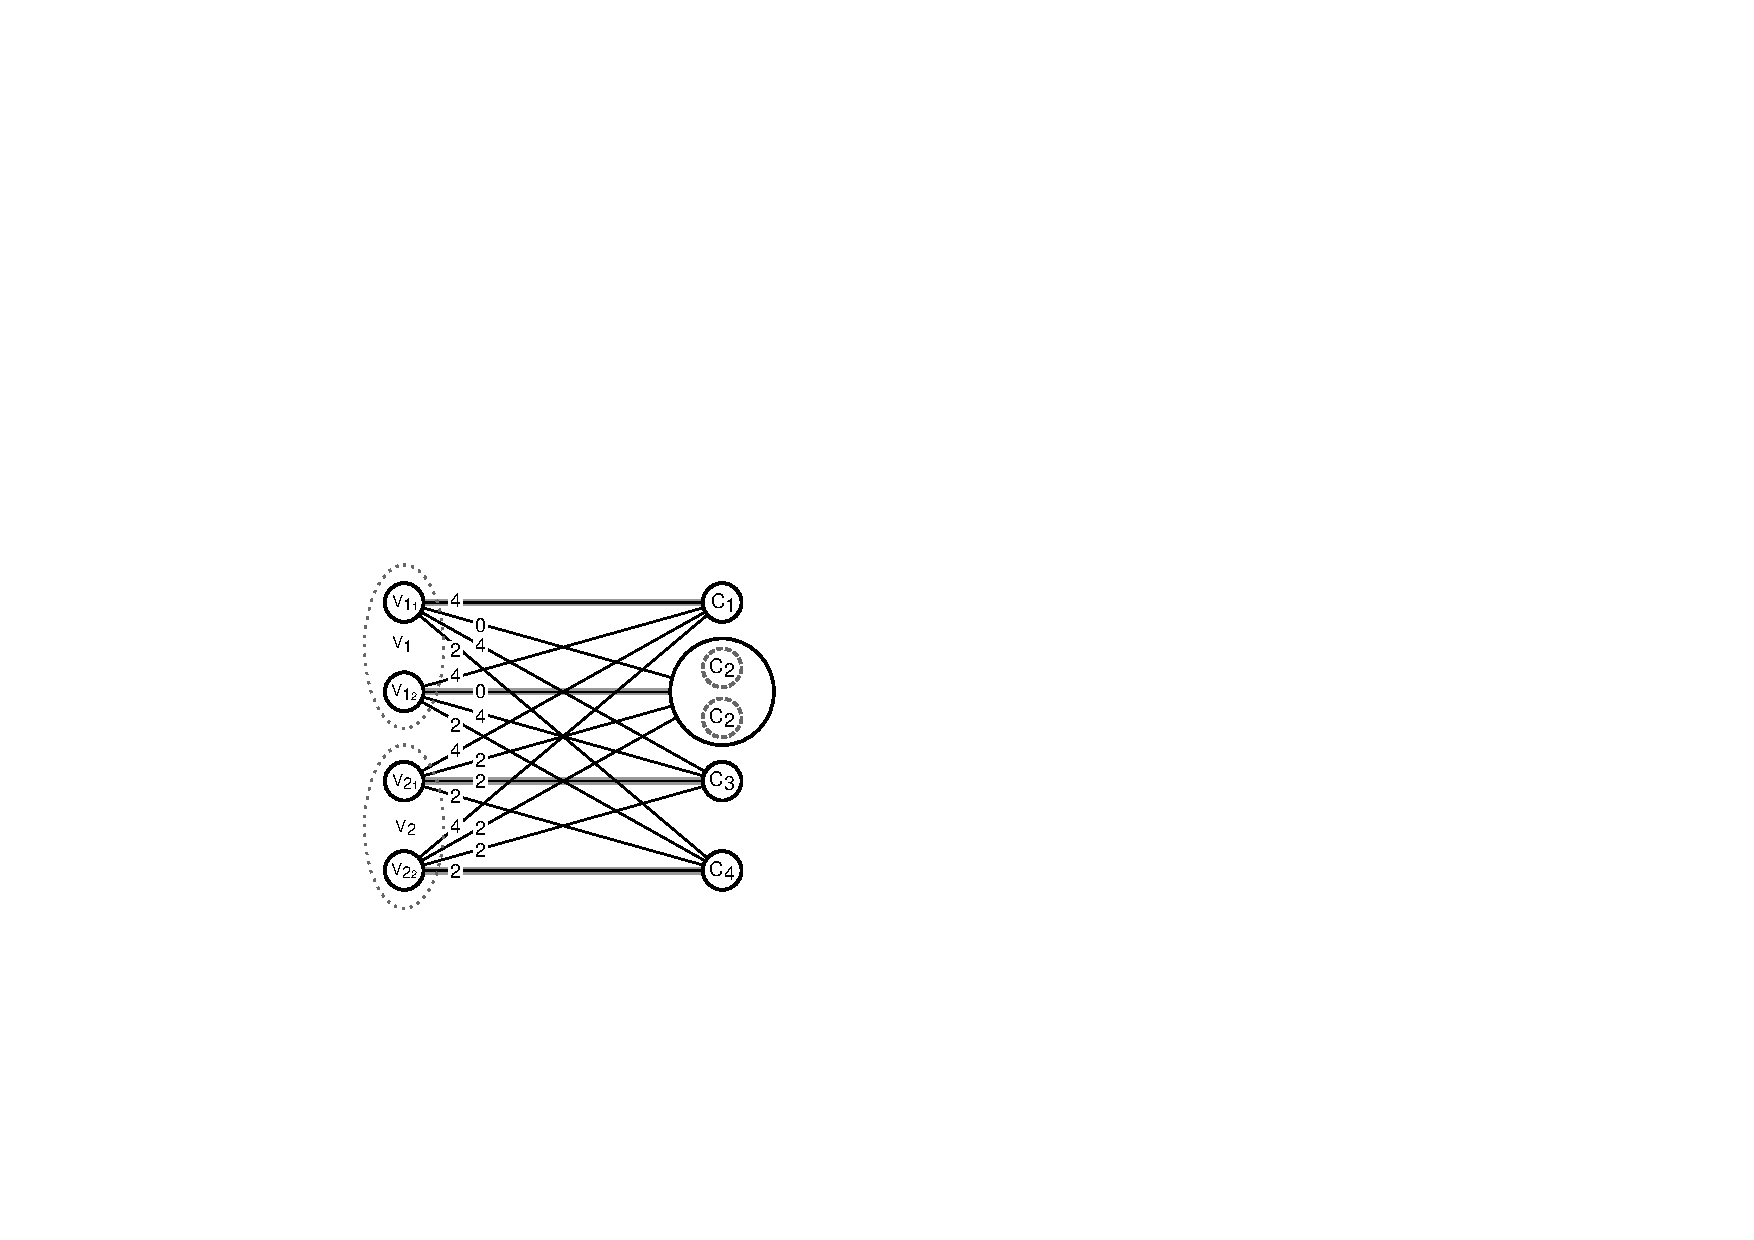
\includegraphics[width = \columnwidth]{figs/matching}
\caption{The matching problem for the instance from
Figure~\ref{fig:model_combined} without $cv$. The solution is indicated by
shadowed lines.}
\label{fig:matching}
\end{minipage}
\end{figure}

Figure~\ref{fig:matching_basic} shows an example of this for the instance from
Figure~\ref{fig:basic_problem}: $\NodeMapping(\VirtualNode_1)$ is four hops
away from all chunks - in the matching problem, this is depicted by the edge
weight on the edges, from $\VirtualNode_1$. $\NodeMapping(\VirtualNode_2)$ is
two hops away from $\Chunk_2$, and 4 hops away from $\Chunk_1$. Hence the
weight of the edge $(\NodeMapping(\VirtualNode_2),\Chunk_2)$ is $2$, while the
weight on the edge to $\Chunk_1$ is $4$. The solution to the minimum weight
perfect bipartite matching contains the edges $(\NodeMapping(\VirtualNode_1),
\Chunk_1)$ and $(\NodeMapping(\VirtualNode_2),
\Chunk_2)$, which is excatly the Chunk to VM assignment $\VmChunkAssignment$
which we identified as an optimal solution in Section~\carlo{TODO}.


This approach can also be used to solve instance of $\Problem$, which have the
$ma$ or $r$ property - or even both.
To Account for the $ma$ property, a single VM has to process exactly
$\MaFactor$ VMs. Hence we can clone a VM to be represented by $\MaFactor$ Nodes.
In order to incorporate the different
replicas of the chunks, we depict all copies of a given $\ChunkTypes$ in a
single %$\ChunkType$
node. We connect each VM to all $\ChunkTypes$ using the
lowest hop count to one of the copies as the weight.

Figure~\ref{fig:matching} illustrates this for the scenario from
Figure~\ref{fig:model_combined} without the $cv$ property: The $2$ VMs are
cloned into $\MaFactor = 2$ VMs each - resulting in a total of $4$ VM nodes in
the matching problem. The $\RedundancyFactor = 2$ chunks of each chunk type are
aggreated $\Chunk_j$ into a single chunk type node in the matching problem -
resulting in a total of $4$ chunk type nodes in the matching graph. The weight
on the edges between all clones of a specific VM and a chunk type are set to
the minimum distance. This can for instance be observed at the egdes connecting
the two clones of $\VirtualNode_1$ to $\Chunk_2$: both weights are 0.



Many algorithms solve the minimum weith perfect matching problem on bipartite
graphs. The algorithms runtimes depend on  the number of nodes in the
graph $n$, the number of edges in the graph $m$, and the largest magnitude of
an edge weight $N$. An efficient algorithm is described by Gabow et al. in
\cite{gabow_scaling_algorithm} and provides a runtime of $\mathcal{O}(n^{3/4}
\cdot m \cdot \log N)$ which translates to $\mathcal{O}((\MaFactor \cdot \Vms +
\ChunkTypes)^{3/4} \cdot  \MaFactor \cdot \Vms \cdot \ChunkTypes \cdot \log
(2 \cdot h(\Tree)))$, where $h(T)$ denotes the height of the tree.

\subsection{Flow based solutions}

A second fundamental algorithm to which many embedding problems can be reduced
to are flow algorithms. We can solve instances of $\Problem$ where the
properties $cv$, $bw$, $r$ and $ma$ are present, by reducing it to a series of
flow problems on an extended host graph. We utilize the following observations:

\newcommand{\Source}{\ensuremath{s}}
\newcommand{\Sink}{\ensuremath{t}}

\begin{enumerate}
\item $cv$ + $bw$ + $r$ + $ma$ degenerates to  $bw$ + $r$ + $ma$.
The placement of the VMs is given. The bandwdith function $\Capacity$ assigns
each edge in the host graph $\SubstrateEdge_i$ a capacity
$\Capacity(\SubstrateEdge_i)$. Since the
host graph is a tree, there exists only one path between two nodes, and hence
it is known how much bandwidth has to be allocated on which links, in oder to
satisfy the communication between the VMs. We can therefore construct a
problem with $bw$ + $r$ + $ma$ which has the same solutions, by defining
$\Capacity'(\SubstrateEdge_i)$ as
$\Capacity(\SubstrateEdge_i) - \textsc{CV}(\SubstrateEdge_i)$, where
$\textsc{CV}(\SubstrateEdge_i)$ denotes the amount which
had to be allocated on the link $\SubstrateEdge_i$ for the communication
between the $\VM s$. If any of the resulting edge capacities is negative, the
instance of $\Problem$ is infeasible.
\item The required bandwidth $\CostTrans$ between each chosen chunk and the
assigned VM of a given $\VC$ is
the same and the pathes to the VMs have to be embedded as unsplittable
pathes.

TODO: rethink if normalization allows solving the problem by integer min-cost-max flow

Hence, all edge capacities in can be normalized to $\CostTrans = 1$.
\item For a (by model) fixed node mapping $\NodeMapping$ and a given chunks to
vm assignment $\VmChunkAssignment$, the computation of a cost
optimal link mapping can be transformed to an integral minimal cost multi-commodity
flow problem, where each VM $\VirtualNode_i$ has a flow demand of $1$ to each
of its assigned chunks $\VmChunkAssignment(\VirtualNode_i)$. This problem can
again be transformed into a integral minimum cost single commodity flow problem
in the following way:
We introduce a
super source $\Source$ and edges $\SubstrateEdge_i^+ = (\Source,
\NodeMapping(\VM_i))$ for
$i \in \{1,\dots,\Vms\}$ with $\Capacity(\SubstrateEdge_i^+) = \MaFactor$,
which connects $\Source$
to the nodes in the host graph, on which the VMs are located.
In addition we create a super sink $\Sink$ and edges $\SubstrateEdge_j^- =
(\VmChunkAssignment(\ChunkLocation(\Chunk_j)), \Sink)$ with capacities
$\Capacity(\SubstrateEdge_j^-) = 1$, which connect the leaves on which the
chunks are located to the sink. In this graph we ask for a flow $f$
of value $\ChunkTypes$ from $\Source$ to $\Sink$. \carlo{TODO: The
equivalency...}
\item The replica selection problem can be integrated into the above described
minimum cost integral single commodity flow problem. Since $\VmChunkAssignment$
is not given, but subject to optimization, the edges connecting $\Sink$ to the
chosen chunks are no longer implementable. Instead, we create a meta node
$\SubstrateNode_{\Chunk_j}$ for each chunk type
$\Chunk_j$ and connect it with \carlo{TODO Check directed?!?} edges
$\SubstrateEdge_{\Chunk_j}^k = (\SubstrateNode_{\Chunk_j},
\VmChunkAssignment(\Chunk_{j_k}))$ for all $k \in
\{1,\dots,\RedundancyFactor\}$. Subsequently we connect the super sink
$\Sink$ to these meta nodes, via
edges $\SubstrateEdge_j^- = (\SubstrateNode)$ with
$\Capacity(\SubstrateEdge_j^-) = 1$. If an integral minimum cost flow $\hat f
: \SubstrateEdges \rightarrow \mathbb{N}$ of value $\ChunkTypes$ exists, it
enters the graph at leaves the graph at $\Sink$. Since the only
edges which connect to $\Sink$ are introduced by our construction $\sum_{j\in
\{1,\dots,\ChunkTypes\}} \hat f(\SubstrateEdge_j^-) = \ChunkTypes$ holds. From
$\Capacity(\SubstrateEdge_j^-) = 1$, follows $\hat f(\SubstrateEdge_j^-) = 1 ~
\forall j \in \{1,\dots, \ChunkTypes\}$. Hence, for each chunk type $\Chunk_j$,
$\sum_{k \in \{0,\dots,\RedundancyFactor\}}\hat f(\SubstrateEdge_{c_j}^k) = 1$
holds, which - due to the integral solution to the minimal cost flow problem -
can be interpreted as the replica selection. $\hat f$ enters the graph at
$\Source$ resulting in $\sum_{i \in \{1,\dots,\Vms\}}\hat f(\SubstrateEdge_i^+)
= \ChunkTypes = \Vms \cdot \MaFactor$. Due to the capacity limitations this is
equivalent to $\hat f(\SubstrateEdge_i^+) = \MaFactor ~ \forall i \in
\{1,\dots, \Vms\}$, which represents $\MaFactor$ outgoing flows for each node
in the host graph, to which a VM is assigned.
\item To compute $\VmChunkAssignment$ from $\hat f$, we process $\hat f$ in the
following way: We chose an aribtrary path $\Path =
\{\SubstrateEdge_{1}, \dots, \SubstrateEdge_{n}\}$, with $\SubstrateEdge_{1} =
(\Source, \NodeMapping(\VirtualNode_i))$, $\SubstrateEdge_{n} =
(\SubstrateNode_j, \Sink)$, $\SubstrateEdge_k= (\SubstrateNode_x,
\SubstrateNode_y) \rightarrow \SubstrateEdge_{k+1} = (\SubstrateNode_y,
\SubstrateNode_z)$, and $\hat f(\SubstrateEdge)\geq 1 ~ \forall \SubstrateEdge
\in \Path$. This is a connected path from the source, to the sink, which has
flow associated on every edge. We set $\VmChunkAssignment(\Chunk_j) =
\VirtualNode_i$ and reduce $\hat f$ on every edge $\SubstrateEdge \in \Path$ by
one. This is repeated, until $|\hat f| = 0$. Due to the tree properties of
$\Tree$, that there is only one path between two nodes, all VM chunk
assignments generated in this value will have the same overall costs.

\begin{comment}
\item For a given chunk \textit{type} to VM assignment, the replica selection
problem
can be integrated into this problem, by introducing nodes
$\SubstrateNode_\ChunkType$ for each
chunk type $\ChunkType$ and connect these nodes via edges
$\SubstrateEdge_\ChunkType = (\SubstrateNode_\ChunkTypes, \SubstrateNode_i)$
for all $i$ such that \carlo{Check macieks part for assigned = true}. The
capacity of all of these edges is set to
$\Capacity(\SubstrateEdge_\ChunkTypes) = 1$. In this problem
%
This problem can be converted into
a integral minimum cost single commodity flow problem,
%
In addition we create a super sink
$\Sink$ and edges
$\SubstrateEdge_\ChunkType^-$ with $\Capacity(\SubstrateEdge_\ChunkType^-) = 1$
%
\item The chunk to vm assignment decision, can be
integrated into the above described flow problem, by transforming it into a
integral minimum cost single commodity flow problem.
We introduce a super source $\Source$ and edges $\SubstrateEdge_i^+ = (\Source,
\NodeMapping(\VM_i))$ for $i \in \{1,\dots,\Vms}$ with
$\Capacity(\SubstrateEdge_i^+) = \MaFactor$, which
connects $\Source$ to the nodes in the host graph, to which the VMs are mapped.
In addition we create a super sink $\Sink$ and edges
$\SubstrateEdge_\ChunkType^-$ with $\Capacity(\SubstrateEdge_\ChunkType^-) = 1$
%
We extend the flow graph with a nodes $\SubstrateNode_\ChunkType$ for each
chunk type $\ChunkType$ and connect these nodes via edges
$\SubstrateEdge_\ChunkType = (\SubstrateNode_\ChunkTypes, \SubstrateNode_i)$
for all $i$ such that \carlo{Check macieks part for assigned = true}. The
capacity of all of these edges is set to
$\Capacity(\SubstrateEdge_\ChunkTypes) = 1$.
In addition we create a super sink $\Sink$ and edges
$\SubstrateEdge_\ChunkType^-$ with $\Capacity(\SubstrateEdge_\ChunkType^-) =
1$, to connect the meta nodes for each chunk type to the super sink.
%Instead of connecting
%$\Source$ to the nodes, to which the VMs are mapped, we connect $\Source$ to
%\textit{all leaves} in the host graph via edges $e_\Leaf^+ = (\Source,
%\SubstrateNode)$. $\Capacity(e_\SubstrateNode^+)$ is set to one, since by
%the definition of our model, only one VM may be mapped to one server. If a
%feasible flow $f : \SubstrateEdges \rightarrow \mathbb{N}$ of value $\Vms$
%exists, then $\Sum_{\Leaf \in \Leaves}$
\end{comment}
\end{enumerate}

\begin{figure}
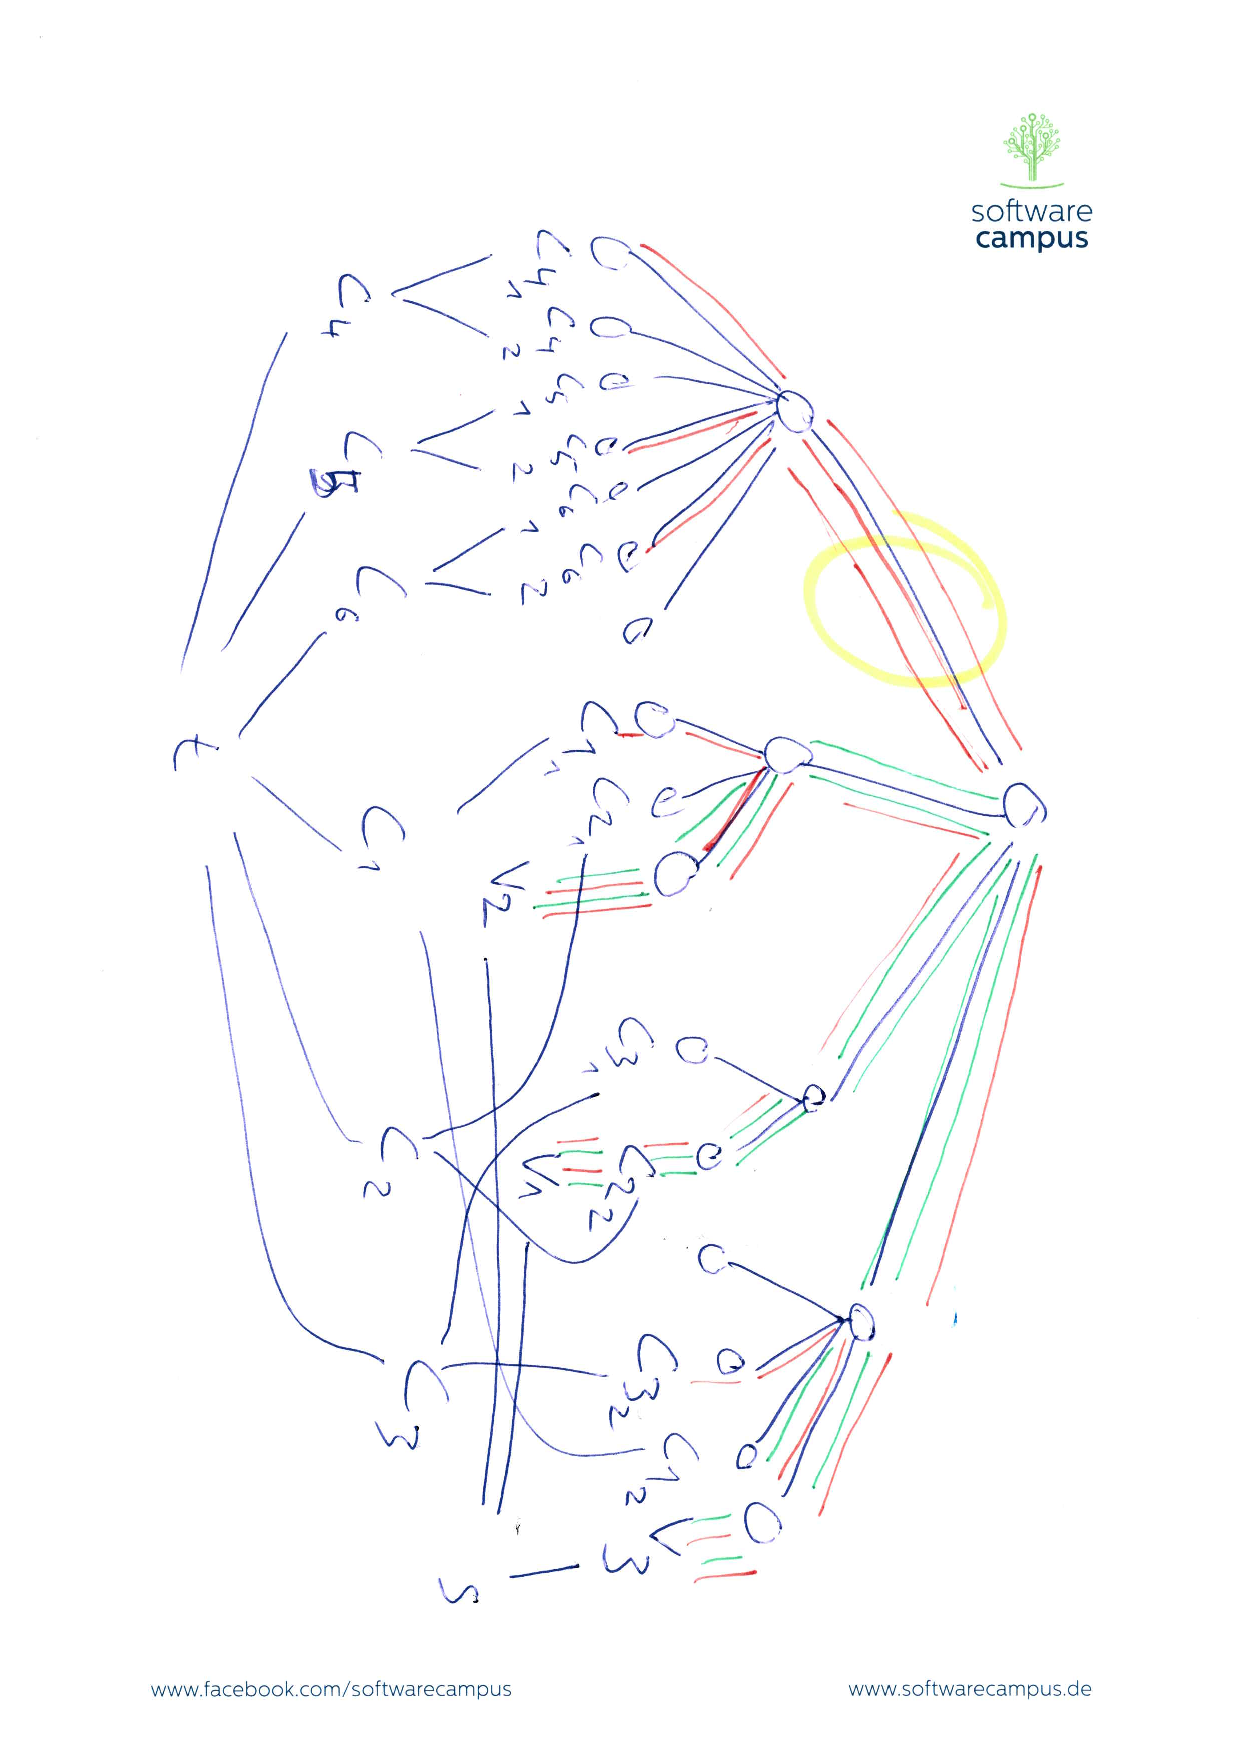
\includegraphics[angle=90,origin=c, height=7cm]{figs/model_fig_skteches/flow}
\end{figure}


Many algorithm can compute a solution for the integral minimum cost maximum
flow problem. One example is the \textit{successive shortest path algorithm},
which can compute a solution in $\mathcal{O}(n \cdot U((n+m)\log n)
)$ time \cite{successive_shortest_path_complexity}, where $n$ is the number of
nodes in the flow graph ($|\SubstrateNodes| + \ChunkTypes$), $m$ is the number
of edges in the substrate graph ($|\SubstrateEdges| + \Vms + \RedundancyFactor
\cdot \ChunkTypes$) and $U$ is the highest capacity in the substrate
($\max(\Capacity(\SubstrateEdge))~\SubstrateEdge\in\SubstrateEdges$).




\begin{comment}
\paragraph{FLOW Construction}

This section presents a flow based solution for the variant of the model which
has bandwidth limitations, communicatin between the $\VM s$ and redundant
$\Chunk s$.

We start by showing that $cv$ + $bw$ + $r$ is the same problem as $bw$ + $r$.
The placement of the $\VM s$ is given. The bandwdith function $b$ assigns
each link in the physical substrate $l_i$ a capacity $c_i$. Since the phyiscal
stubstrate is a tree there exists only one path between two nodes, and hence it
is known how much bandwidth has to be allocated on which links, in oder to
satisfy the communication between the $\VM s$. We can therefore construct a
problem with $bw$ + $r$ which has the same solutions, by defining $b'(l)$ as
$b(l) - cv_l$, where $cv_l$ denotes the amount which had to be allocated on the
link $l$ for the communication between the $\VM s$.

To construct the flow graph, we start from the physical
substrate. Each edge has a associated costs of $1$ and bandwidth according the
available bandwidth due to the distribution provided by the $b$ function of the
$bw$ property of the model. In addition we create and a node for each
$\ChunkType$. Each of these nodes is connected to every node in the physical
topology, which has a $\Chunk$ of the corresponding type. The capacity of these
edges is $1$ and the costs are $0$. In addition we create the source, and
connect it to all nodes, which represent $\ChunkType s$. The capacity of the
edges from the sink is $1$ and it's costs are $0$.
On this flow graph, we now solve the (integer) Max-Flow-Min-Cost Problem.

If the resulting maximal flow $\hat f$ has a value $|\hat f|< |C| = |V_V|$, the
$\Problem$ is infeasible - otherwise we can construct a solution from $\hat f$.
To construct the solution we choose an arbitrary path $p = \{e_1,\dots,
e_n\}$ \carlo{TODO check n}, such that $f(e_i) > 1 ~ \forall i \in
\{1,\dots,n\}$.
\end{comment}

%\subsection{Dynamic programming solution}

\subsection{Dynamic programming based solutions}

Dynamic programming is an algorithmic paradigm, which can be exploited in
order to solve instances of $\Problem$, which contain the properties $fp$ +
$cv$ + $ma$ and $bw$. This section will describes an dynamic programming based
algorithm which solves $fp$ + $cv$ + $bw$, and points out how to extend or
reduce it to other combinations of properties.

\maciek{TODO: if we ever want to put 2 replica NP-completeness proof, we need
to introduce idle machines}

\maciek{TODO: here we need to explicitly say what we mean by mixing MA and idle
machines; just as a reminder, we decided to force the machines to be full or
empty}

%\subsection{new}

\newcommand{\Opt}{\ensuremath{Opt}}
\newcommand{\Children}{\ensuremath{children}}
%\newcommand{\Cost}{\ensuremath{\textsc{cost}}}

\newcommand{\Uplink}{\ensuremath{\textsc{uplink}}}
\newcommand{\ChunkCount}{\ensuremath{\textsc{cis}}}
\newcommand{\VmCount}{\ensuremath{\textsc{vis}}}
\newcommand{\Right}{\ensuremath{r}}
\newcommand{\InverseAssignment}{\ensuremath{\VmChunkAssignment^{-1}}}

Our dynamic programming approach depends heavyly on the fact that, given the
amounts of VMs and Chunks in a given subtree $\Tree' \subset \Tree$, the
bandwidth costs of an optimal assignment $\VmChunkAssignment$ on
$\Uplink(\SubstrateNode')$, where $\SubstrateNode'$ is the root of $\Tree'$,
can be computed efficiently. To show this, we have to introduce two aditional
functions: $\ChunkCount : \SubstrateNodes
\rightarrow
2^\Chunks$ yields which chunks are located in the subtree where the root node
is the argument. The evaluation of $\ChunkCount$ can be done in a
simple bottom
up manner: All leaf nodes $\Leaf_i$ are initialized with $\ChunkCount(\Leaf_i)
= \{\Chunk_j\}$ if a chunk is present at $\Leaf_i$ ($\exists ~ \Chunk_j \in
\Chunks : \ChunkLocation(\Chunk_j) = \Leaf_i \Leftrightarrow
\ChunkCount(\Leaf_i) = \{\Chunk_j\}$), and with $\ChunkCount(\Leaf_i) =
\emptyset$ otherwise ($\ChunkLocation(\Chunk_j) \neq \Leaf_i \forall \Chunk_j
\in
\Chunks \Leftrightarrow \ChunkCount(\Leaf_i) = \emptyset$). On every non-leaf
node $\SubstrateNode_i \in \SubstrateNodes / \Leaves$, $\ChunkCount$ is equal
to the union of the childrens' $\ChunkCount$s
($\ChunkCount(\SubstrateNode_i)
= \bigcup_{\SubstrateNode_k \in \Children{\SubstrateNode_i}}
\ChunkCount(\SubstrateNode_k)$). In addition we introduce a second function
$\VmCount : \SubstrateNodes \rightarrow 2^{\VirtualNodes}$, which stores for
every node $\SubstrateNode'$, which VMs are present in the subtree $\Tree'$
with the root $\SubstrateNode'$. $\VmCount$ can be evaluted in the
same bottom-up fashion as $\ChunkCount$.

For the efficient computation it is
important to show, that an optimal assignment will always assign chunks to VMs
in the same subtree - if possible. More formally we proove that the following
corollary holds for the transport costs $\Cost_T$:

\subsubsection{Without MA}

\begin{corollary}
\label{corollary:local_matching}
For a given VM mapping $\NodeMapping$ and any subtree $\Tree' \subseteq
\Tree$ with the root $\SubstrateNode'$, which contains $n =
|\ChunkCount(\SubstrateNode')|$ chunks and $m = |\VmCount(\SubstrateNode')|$
VMs, the bandwidth costs of an optimal assignment $\VmChunkAssignment$ for
transferring the chunks to the VMs ($\Cost_T$
component) on $\Uplink(\SubstrateNode')$ are $|n
- m| \cdot \CostTrans$.
\end{corollary}

To show Corollary~\ref{corollary:local_matching}, we will use two lemmas, which
cover the cases $|\ChunkCount(\SubstrateNode')| \geq
|\VmCount(\SubstrateNode')|$ and $|\ChunkCount(\SubstrateNode')| \leq
|\VmCount(\SubstrateNode')|$ - showing that an optimal assignment
$\VmChunkAssignment$, will assign chunks locally (i.e. to VMs in the
same subtree). All chunks which cannot be served locally will be served in
other subtrees, resulting in the transport costs on $\Uplink(\SubstrateNode')$
described in Corollary~\ref{corollary:local_matching}. When the amount of VM
exceeds the amount of chunks in $\Tree'$, the transport costs will still occur,
since some chunks $\Chunk_j \notin \ChunkCount(\SubstrateNode')$ will have to
be transported to the VMs in $\VmCount(\SubstrateNode')$, which cannot be
assigned to chunks in $\ChunkCount(\SubstrateNode')$.

\begin{lemma}
\label{lemma:matching1}
For a given VM mapping $\NodeMapping$ and any subtree $\Tree' \subseteq
\Tree$ with the root $\SubstrateNode'$, which contains at least one VM per
chunk $|\ChunkCount(\SubstrateNode')| \leq |\VmCount(\SubstrateNode')$, an
optimal chunk to VM assignment $\VmChunkAssignment$, cannot assign a chunk
to a VM outside of $\Tree'$ ($\VmChunkAssignment(\Chunk_j) \in
\VmCount(\SubstrateNode')~ \forall \Chunk_j \in \ChunkCount(\SubstrateNode')$).
\end{lemma}

\begin{proof}
 By contradiction. Assume $\VmChunkAssignment$ is an optimal chunk to vm
assignment $\VmChunkAssignment$ with $\VmChunkAssignment(\Chunk_j)
=\VirtualNode_l \notin \VmCount(\SubstrateNode')$. $\VmChunkAssignment$ assigns
the property for any subtree $\Tree'$. From $|\ChunkCount(\SubstrateNode')|
\geq
|\VmCount(\SubstrateNode')|$ follows that there is at least one
combiantion of
VM
$\VirtualNode_m \in \VmCount(\SubstrateNode')$ and chunk $\Chunk_k \notin
\ChunkCount(\SubstrateNode')$ with $\VmChunkAssignment(\Chunk_k) =
\VirtualNode_m$. Let $\Tree''$ with the root $\SubstrateNode''$ denote the
smallest subtree of $\Tree$ with $\Tree' \subset \Tree'' \subseteq \Tree$ and
$\VirtualNode_l \in \VmCount(\SubstrateNode'')$. We will now show, that an
alternate assignment $\VmChunkAssignment'$ with
$\VmChunkAssignment'(\Chunk_j) = \VirtualNode_m$ and
$\VmChunkAssignment'(\Chunk_k) = \VirtualNode_l$, as lower costs, to generate
the contradiction. We do this, with the following case diffentiation:
\\
\textbf{Case 1:} $\Chunk_k \in \ChunkCount(\SubstrateNode'')$\\
$\Distance(\NodeMapping(\VirtualNode_l), \ChunkLocation(\Chunk_k)) \leq
\Distance(\NodeMapping(\VirtualNode_l), \ChunkLocation(\Chunk_j)$ and
$\Distance(\NodeMapping(\VirtualNode_m), \ChunkLocation(\Chunk_j)) <
\Distance(\NodeMapping(\VirtualNode_m), \ChunkLocation(\Chunk_k)$. Due to the
direct correlation of $\CostPerChunk$ and $\Distance$, exchanging the
assignment of $\Chunk_j$ and $\Chunk_k$ will reduce the overall costs, since
$\CostPerChunk(\VirtualNode_m)$ will be reduced,
$\CostPerChunk(\VirtualNode_l)$ cannot be increased, and the other components
of the costs remain unchanged. As a result $\VmChunkAssignment'$ has lower
costs than $\VmChunkAssignment$, which is in contraction, to the optimality of
$\VmChunkAssignment$.\\
\textbf{Case 2:} $\Chunk_k \notin \ChunkCount(\SubstrateNode'')$\\
Since $\Tree$ is balanced we get $\Distance(\NodeMapping(\VirtualNode_m),
\ChunkLocation(\Chunk_k)  = \Distance(\NodeMapping(\VirtualNode_l),
\ChunkLocation(\Chunk_k)$. In addition $\Distance(\NodeMapping(\VirtualNode_l,
\Chunk_j)) > \Distance(\NodeMapping(\VirtualNode_m,
\Chunk_j)) $ holds, since $\VirtualNode_m \in \VmCount(\SubstrateNode')$ and
$\VirtualNode_l \notin
\VmCount(\SubstrateNode')$. Hence swapping the assignment of $\Chunk_j$ and
$\Chunk_k$ will reduce $\CostPerChunk(\Chunk_j)$, and keep all other costs
stable. This however is in contraction to the cost optimality of
$\VmChunkAssignment$, since $\VmChunkAssignment'$ would be cheaper.
\end{proof}

\begin{lemma}
\label{lemma:matching2}
For a given VM mapping $\NodeMapping$ and any subtree $\Tree' \subseteq
\Tree$ with the root $\SubstrateNode'$, which contains at least one Chunk per
VM $|\ChunkCount(\SubstrateNode')| \geq |\VmCount(\SubstrateNode')$, an
optimal chunk to VM assignment $\VmChunkAssignment$, cannot assign a chunk
which is not in $\ChunkCount(\SubstrateNode')$ to a VM in
$\VmCount(\SubstrateNode')$ ($\VmChunkAssignment(\Chunk_j) \in
\VmCount(\SubstrateNode')~ \rightarrow \Chunk_j \in
\ChunkCount(\SubstrateNode')$).
\end{lemma}

\begin{proof}
 Analog to Lemma~\ref{lemma:matching1}
\end{proof}

If the $cv$ property is present in our model, transportation costs might not be
the only costs, which occur on $\Uplink(\SubstrateNode')$. The second cause of
bandwidth costs, are the inter VM communication cost $\Cost_C$.

\begin{corollary}
\label{corollary:comCost}
 For a given VM mapping $\NodeMapping$ and any subtree $\Tree' \subseteq
\Tree$ with the root $\SubstrateNode'$, which contains $n
= |\VmCount(\SubstrateNode')|$ VMs, the communication costs ($\Cost_C$
component) on
$\Uplink(\SubstrateNode')$ are $n \cdot (\Vms - n)
\cdot
\CostCom$.
\end{corollary}

\begin{proof}
Due to the fact the nodemapping is given, the enpoints of the communication
pathes are known. Since $\Tree$ is a tree, there exists only one path between
two nodes in the substrate. These pathes do not contain the
$\Uplink(\SubstrateNode')$ if, both VMs are mapped to nodes in $\Tree'$.
However, each of the $n$ VMs inside $\Tree'$ has to communicate with each VM
outside of $\Tree'$. The number of VMs outside of $\Tree$ is the total number
of VMs, minus the amount of VMs inside $\Tree'$, resulting in $n \cdot (\Vms -
n)$ communications - which each inflict $\CostCom$ bandwidth costs.
\end{proof}

\subsubsection{With MA}

\begin{corollary}
\label{corollary:local_matching}
For a given VM mapping $\NodeMapping$ and any subtree $\Tree' \subseteq
\Tree$ with the root $\SubstrateNode'$, which contains $n =
|\ChunkCount(\SubstrateNode')|$ chunks and $m = |\VmCount(\SubstrateNode')|$
VMs, the bandwidth costs of an optimal assignment $\VmChunkAssignment$ for
transferring the chunks to the VMs ($\Cost_T$
component) on $\Uplink(\SubstrateNode')$ are $|n\cdot\MaFactor
- m| \cdot \CostTrans$.
\end{corollary}

To show Corollary~\ref{corollary:local_matching}, we will use two lemmas, which
cover the cases $|\ChunkCount(\SubstrateNode')| \geq
|\VmCount(\SubstrateNode')| \cdot \MaFactor$ and
$|\ChunkCount(\SubstrateNode')| \leq
|\VmCount(\SubstrateNode')| \cdot \MaFactor$ - showing that an optimal
assignment
$\VmChunkAssignment$, will assign chunks locally (i.e. to VMs in the
same subtree). All chunks which cannot be served locally will be served in
other subtrees, resulting in the transport costs on $\Uplink(\SubstrateNode')$
described in Corollary~\ref{corollary:local_matching}. When the amount of
available $\VmSlots$
exceeds the amount of chunks in $\Tree'$, the transport costs will still occur,
since some chunks $\Chunk_j \notin \ChunkCount(\SubstrateNode')$ will have to
be transported to the VMs in $\VmCount(\SubstrateNode')$, which have $\VmSlots$
which cannot be
assigned to chunks in $\ChunkCount(\SubstrateNode')$.

\begin{lemma}
\label{lemma:matching1}
For a given VM mapping $\NodeMapping$ and any subtree $\Tree' \subseteq
\Tree$ with the root $\SubstrateNode'$, which contains at least one $\VmSlot$
per
chunk $|\ChunkCount(\SubstrateNode')| \leq |\VmCount(\SubstrateNode')| \cdot
\MaFactor$, an
optimal chunk to VM assignment $\VmChunkAssignment$, cannot assign a chunk
to a VM outside of $\Tree'$ ($\VmChunkAssignment(\Chunk_j) \in
\VmCount(\SubstrateNode')~ \forall \Chunk_j \in \ChunkCount(\SubstrateNode')$).
\end{lemma}

\begin{proof}
 By contradiction. Assume $\VmChunkAssignment$ is an optimal chunk to vm
assignment $\VmChunkAssignment$ with $\VmChunkAssignment(\Chunk_j)
=\VirtualNode_l \notin \VmCount(\SubstrateNode')$. $\VmChunkAssignment$ assigns
the property for any subtree $\Tree'$. From $|\ChunkCount(\SubstrateNode')|
\geq
|\VmCount(\SubstrateNode')| \cdot \MaFactor$ follows that there is at least one
combiantion of
VM
$\VirtualNode_m \in \VmCount(\SubstrateNode')$ and chunk $\Chunk_k \notin
\ChunkCount(\SubstrateNode')$ with $\VmChunkAssignment(\Chunk_k) =
\VirtualNode_m$. Let $\Tree''$ with the root $\SubstrateNode''$ denote the
smallest subtree of $\Tree$ with $\Tree' \subset \Tree'' \subseteq \Tree$ and
$\VirtualNode_l \in \VmCount(\SubstrateNode'')$. We will now show, that an
alternate assignment $\VmChunkAssignment'$ with
$\VmChunkAssignment'(\Chunk_j) = \VirtualNode_m$ and
$\VmChunkAssignment'(\Chunk_k) = \VirtualNode_l$, as lower costs, to generate
the contradiction. We do this, with the following case diffentiation:
\\
\textbf{Case 1:} $\Chunk_k \in \ChunkCount(\SubstrateNode'')$\\
$\Distance(\NodeMapping(\VirtualNode_l), \ChunkLocation(\Chunk_k)) \leq
\Distance(\NodeMapping(\VirtualNode_l), \ChunkLocation(\Chunk_j)$ and
$\Distance(\NodeMapping(\VirtualNode_m), \ChunkLocation(\Chunk_j)) <
\Distance(\NodeMapping(\VirtualNode_m), \ChunkLocation(\Chunk_k)$. Due to the
direct correlation of $\CostPerChunk$ and $\Distance$, exchanging the
assignment of $\Chunk_j$ and $\Chunk_k$ will reduce the overall costs, since
$\CostPerChunk(\VirtualNode_m)$ will be reduced,
$\CostPerChunk(\VirtualNode_l)$ cannot be increased, and the other components
of the costs remain unchanged. As a result $\VmChunkAssignment'$ has lower
costs than $\VmChunkAssignment$, which is in contraction, to the optimality of
$\VmChunkAssignment$.\\
\textbf{Case 2:} $\Chunk_k \notin \ChunkCount(\SubstrateNode'')$\\
Since $\Tree$ is balanced we get $\Distance(\NodeMapping(\VirtualNode_m),
\ChunkLocation(\Chunk_k)  = \Distance(\NodeMapping(\VirtualNode_l),
\ChunkLocation(\Chunk_k)$. In addition $\Distance(\NodeMapping(\VirtualNode_l,
\Chunk_j)) > \Distance(\NodeMapping(\VirtualNode_m,
\Chunk_j)) $ holds, since $\VirtualNode_m \in \VmCount(\SubstrateNode')$ and
$\VirtualNode_l \notin
\VmCount(\SubstrateNode')$. Hence swapping the assignment of $\Chunk_j$ and
$\Chunk_k$ will reduce $\CostPerChunk(\Chunk_j)$, and keep all other costs
stable. This however is in contraction to the cost optimality of
$\VmChunkAssignment$, since $\VmChunkAssignment'$ would be cheaper.
\end{proof}

\begin{lemma}
\label{lemma:matching2}
For a given VM mapping $\NodeMapping$ and any subtree $\Tree' \subseteq
\Tree$ with the root $\SubstrateNode'$, which contains at least one Chunk per
$\VmSlot$ $|\ChunkCount(\SubstrateNode')| \geq |\VmCount(\SubstrateNode')|
\cdot \MaFactor$, an
optimal chunk to VM assignment $\VmChunkAssignment$, cannot assign a chunk
which is not in $\ChunkCount(\SubstrateNode')$ to a VM in
$\VmCount(\SubstrateNode')$ ($\VmChunkAssignment(\Chunk_j) \in
\VmCount(\SubstrateNode')~ \rightarrow \Chunk_j \in
\ChunkCount(\SubstrateNode')$).
\end{lemma}

\begin{proof}
 Analog to Lemma~\ref{lemma:matching1}
\end{proof}

If the $cv$ property is present in our model, transportation costs might not be
the only costs, which occur on $\Uplink(\SubstrateNode')$. The second cause of
bandwidth costs, are the inter VM communication cost $\Cost_C$.

\begin{corollary}
\label{corollary:comCost}
 For a given VM mapping $\NodeMapping$ and any subtree $\Tree' \subseteq
\Tree$ with the root $\SubstrateNode'$, which contains $n
= |\VmCount(\SubstrateNode')|$ VMs, the communication costs ($\Cost_C$
component) on
$\Uplink(\SubstrateNode')$ are $n \cdot (\Vms - n)
\cdot
\CostCom$.
\end{corollary}

\begin{proof}
Due to the fact the nodemapping is given, the enpoints of the communication
pathes are known. Since $\Tree$ is a tree, there exists only one path between
two nodes in the substrate. These pathes do not contain the
$\Uplink(\SubstrateNode')$ if, both VMs are mapped to nodes in $\Tree'$.
However, each of the $n$ VMs inside $\Tree'$ has to communicate with each VM
outside of $\Tree'$. The number of VMs outside of $\Tree$ is the total number
of VMs, minus the amount of VMs inside $\Tree'$, resulting in $n \cdot (\Vms -
n)$ communications - which each inflict $\CostCom$ bandwidth costs.
\end{proof}

%$\ChunkCount_\SubstrateNode$ contains the
%number of chunks at
%or below
%$\SubstrateNode$ and $\Opt_\SubstrateNode[i]~i\in \{0,\dots,\Vms\}$ contains
%the
%total cost ($\CostCom$ + $\CostTrans$) for placing $i$ VMs at or beneath
%$\SubstrateNode$. These costs account for bandwidth costs on
%$\Uplink(\SubstrateNode)$. To denote that it is impossible to place $i$ VMs at
%or beneath $\SubstrateNode$, we set $\Opt_\SubstrateNode[i] = \infty$.
%
%, we generate a
%function $\ChunkCount : \SubstrateNode \rightarrow \mathbb{N}$ and second
\newcommand{\NodesToProcess}{\ensuremath{\textsc{nodesToProcess}}}

\begin{algorithm}[tbhp]
\DontPrintSemicolon % Some LaTeX compilers require you to use
%\dontprintsemicolon instead
\SetAlgoNoEnd
\KwIn{$\SubstrateNode \in \SubstrateNodes$}
\vspace{6pt}
\While{$|\Children(\SubstrateNode) > 2|$}{
  \textbf{set} $\SubstrateNodes \gets \SubstrateNodes \cup
\{\SubstrateNode^*\}$\;
  \textbf{~~with }$\Capacity(\SubstrateNode^*) \gets 0$
  \textbf{ and }$\Cost(\SubstrateNode^*) \gets  1$\;
  \textbf{choose any }$\SubstrateNode'$\textbf{ from
}$\Children(\SubstrateNode)$\;
  $cap \gets \Capacity((\SubstrateNode, \SubstrateNode'))$\;
  $\SubstrateEdges \gets \SubstrateEdges \setminus \{(\SubstrateNode,
\SubstrateNode')\}$\;
  \textbf{set} $\SubstrateEdges \gets \SubstrateEdges \cup \{(\SubstrateNode^*,
\SubstrateNode')\}$\;
  \textbf{~~with }$\Capacity((\SubstrateNode^*, \SubstrateNode')) i\gets cap$
  \textbf{ and }$\Cost((\SubstrateNode^*,\SubstrateNode')) \gets  1$\;
  \textbf{set} $\SubstrateNodes \gets \SubstrateNodes \cup \{(\SubstrateNode^*,
\SubstrateNode)\}$\;
  \textbf{~~with }$\Capacity((\SubstrateNode^*, \SubstrateNode)) i\gets \infty$
  \textbf{ and }$\Cost((\SubstrateNode^*, \SubstrateNode)) \gets  0$\;
  $binarize(\SubstrateNode')$\;
}
\For{\textbf{each } $\SubstrateNode' \in \Children(\SubstrateNode)$}{
  $binarize(\SubstrateNode')$\;
}

\caption{$binarize(\SubstrateNode \in \SubstrateNodes)$}
\label{algo:binarization}
\end{algorithm}








Our dynamic program works on bianry trees. Algorithm~\ref{algo:binarization}
shows the algorithm to recursively binarize a (sub-)tree with the root $v$:
%To binarize tree $\Tree$, we start by processing each vertex $v \in
%\SubstrateNodes$ in the following root to leaf manner:
While $v$ has more than
$2$ children, we choose an arbitrary node $v' \in \Children(v)$
and create a new virtual node $v^*$. We remove the edge $e = (v, v')$ which
connected $v$ to it's child $v'$ from $\SubstrateEdges$. Subsequently we create
a new edge, which connects the
child to the new node $e^*_1 = (v', v^*)$, set it's
$\Cost(e^*_1) = 1$ and it's capacity to the value of the removed edge $e$
($\Capacity(e^*_1) = \Capacity(e)$). Additionally we gerate an edge $e^*_2 =
(v^*, v)$. $\Capacity(e^*_2)$ is $\infty$ and $\Cost{e^*_2}$ is set to $0$.
Subsequently we process the subtree with the root $v'$. If the current node has
two or less children $v$ does not violate the binary constraint, and hence the
binarization process of $v$ is finished. However, it is neccessary to
recursively binarize the subtrees with roots $v'_1, v'_2 \in \Children(v)$, if
they exists.

To compute a solution $\Sol$ for an instance of $\Problem$ we leverage a
function $\Opt : \SubstrateNodes \times \mathbb{N} \rightarrow \mathbb{R}$.
$\Opt$ represents the inflicted bandwidth costs in a subtree $\Tree' \subset
\Tree$ with the root $\SubstrateNode'$, which will occur if $n$ (argument 2)
nodes, will be placed in $\Tree'$.
This
function can be evaluated
efficiently in a bottom up manner. After $\Opt$ is evaluated for the entire
tree, $\Sol$ can be constructed from the values of $\Opt$.
%If $|\Children(v)| > 2$, we choose an arbitrary node $v' \in \Children(v)$
%and create a new virtual node $v^*$. We create a new edge $e^*_1$, set it's
%cost to $1$ and it's capacity to $\Bandwidth(e)$.

%In addition we evaluate a function $\ChunkCount : \SubstrateNodes \rightarrow
%2^\Chunks$, which yields which chunks are located beneath a specific node in
%the host graph. The evaluation of $\ChunkCount$ can be done in a simple
%bottom
%up manner: All leaf nodes $\Leaf_i$ are initialized with
%\ChunkCount(\Leaf_i)
%= \{\Chunk_j\}$ if a chunk is present at $\Leaf_i$ ($\exists ~ \Chunk_j \in
%\Chunks : \ChunkLocation(\Chunk_j) = \Leaf_i \Leftrightarrow
%\ChunkCount(\Leaf_i) = \{\Chunk_j\}$.), and with $\ChunkCount(\Leaf_i) =
%\emptyset$ otherwise ($\ChunkLocation(\Chunk_j) \neq \Leaf_i \forall \Chunk
%\in
%\Chunks \Leftrightarrow \ChunkCount(\Leaf_i) = \emptyset$). On every non-leaf
%node $\SubstrateNode_i \in \SubstrateNodes / \Leaves$, the count count is
%equal
%to the union of the childrens chunk count values
%($\ChunkCount(\SubstrateNode_i)
%= \bigcup_{\SubstrateNode_k \in \Children{\SubstrateNode_i}}
%\ChunkCount(\SubstrateNode_k)$).
On the leaves the initialization of $\Opt$
works in the following way: For $0$ or
$1$ VMs which are placed at the Leaf $\Leaf_i$, we set $\Opt(\Leaf_i, n \in
\{0,1\}) = 0$; for all other amounts of VMs we set $\Opt(\Leaf_i, n \in
\{2,\dots,\Vms\}) = \infty$, to represent that these amount of VMs are
infeasible at or below the leaves.

To recursively compute $\Opt(\SubstrateNode_i, n \in \{0,\dots\Vms\})$ for a
non-leaf node $\SubstrateNode_i \in \SubstrateNodes / \Leaves$, we leverage
Corollaries~\ref{corollary:local_matching} and \ref{corollary:comCost}. Since
we do it in a bottom up manner, $\Opt(\SubstrateNode_c, n)$
is allready evaluated for all $n \in \{0,\dots,\Vms\}$ and all
$\SubstrateNode_c \in \Children(\SubstrateNode_i)$.

Since VMs may only be embded in leaves, the bandwidth costs of placing $n$ VMs
in the subtree $\SubstrateNode_i$ with the childen $\SubstrateNode_l$ and
$\SubstrateNode_r$ can be divided into the costs of placing $l$ VMs in the
subtree with root $\SubstrateNode_l$ , the costs of placing
$r$ VMs in the subtree with $\SubstrateNode_r$, and the costs on the
$\Uplink(\SubstrateNode_l)$ and $\Uplink(\SubstrateNode_r)$. The costs of
placing the VMs beneath the $\SubstrateNode_l$ are allready known from
$\Opt$. \carlo{(New to put an emphasis on charging only two edges...:) The only
additional bandwidth costs on this level of recursion occur on
$\Uplink(\SubstrateNode_l)$ (and $\Uplink(\SubstrateNode_r)$ respectively).}
The costs on $\Uplink(\SubstrateNode_l)$ can again be divided: From
Corollary~\ref{corollary:local_matching}, we know that the transport costs are
 $|\ChunkCount(\SubstrateNode_l) - l| \cdot \CostTrans$ and from
Corollary\ref{corollary:comCost}, we know that the communication costs are
$l\cdot (\Vms - l) \cdot \CostCom$. The same is valid for $\SubstrateNode_r$.
We now iterate over all possible amounts of VMs $n \in \{0,\dots,\Vms\}$ and
try to find the cheapest split of $n$ into $\hat l$ and $\hat r$ with
$\hat l + \hat r = n$ for each $n$. We define $\Opt(\SubstrateNode_i, n) =
\Opt(\SubstrateNode_{l}, \hat l) + \Opt(\SubstrateNode_{r}, \hat r) +
(|\ChunkCount(\SubstrateNode_{l}) - \hat
l|+|\ChunkCount(\SubstrateNode_{r}) - \hat r|) \cdot \CostTrans + (\hat
l\cdot (\Vms - \hat l) + \hat r\cdot (\Vms - \hat r)) \cdot \CostCom$. If the
bandwidth sum on one of the uplinks exceeds the capacity defined by
$\Capacity$, we treat the solution as infeasible, by treating the costs as
$\infty$. Algorithm~\ref{algo:dynAggregation} illustrates this... \carlo{Do you
want to keep this?}

Since the total costs $\sum_{\Chunk_j \in
\Chunks}\Cost(\Chunk_j)$ of an optimal assignment $\VmChunkAssignment$
consists only of $\Cost_T$ and $\Cost_C$, for which $\Opt$ accounts accurately
(Corollaries~\ref{corollary:local_matching} and \ref{corollary:comCost}),
$\Opt(\SubstrateNode, \Vms)$ will be equal to $\sum_{\Chunk_j \in
\Chunks}\Cost(\Chunk_j)$ - or $\infty$ if the instance is infeasible.

\carlo{TODO Construction from $\Opt$ or described how to store? Or say trivial?}

\subsubsection{Algorithm part}

\carlo{I didn't know where you wanted to put this. Feel free to modify / move
it.}

An implementation of our DP based solution can be implemented efficiently,
using the following data structures: $\ChunkCount$ can be
represented by single values on the respective nodes in the host graph. The
node to which it is attached, will replace the argument of $\ChunkCount$: the
values will represent the amount of chunks, which are located in the subtree
with respective node, as root.

$\Opt$ can be realized by an array, which is attached to a node in the host
graph. The node again replaces the first argument. The index of the array, will
replace the second argument of $\Opt$. If a value in the array of node
$\SubstrateNode_i$ at index $i$ is set to a value $x$, this represents, that
placing $i$ VMs in the subtree beneath $\SubstrateNode_i$, will inflict
bandwidth costs of $x$ on the links in the subtree beneath $\SubstrateNode_i$.

Note that $\VmCount$ will not be implemented at all - it is only neccessary for
the former proofs.

\subsubsection{$\Opt = \infty \rightarrow $infeasible}

\carlo{TODO: Move root to model section}

\begin{lemma}
An instance of $\Problem$ is infeasible if $\Opt(\SubstrateNode,\Vms) = \infty$,
where $\SubstrateNode$ is the root of $\Tree$.
\end{lemma}

\begin{proof}
By contraction: Assume the instance of $\Problem$ is feasible and
$\Opt(\SubstrateNode,\Vms) = \infty$. This menas a node mapping $\NodeMapping$
and an assignment $\VmChunkAssignment$ exists, which do not violate the
bandwidth capacities on all edges in $\SubstrateEdges$. Since VMs may only be
located at leaves, $\NodeMapping$ will place $r$ VMs in the subtree beneath the
right child of $\SubstrateNode$ and the remaining $\Vms - r$ VMs in the subtree
beneath the other child of $\SubstrateNode$.
$\Opt(\SubstrateNode,\Vms)$ can be $\infty$ due to two reasons, which can occur
at or beneath one of the children of $\SubstrateNode$. Let us without loss of
generality assume that the reason occured beneath the right child. The first
reason, is that there is not sufficient bandwidth
$\Capacity(\Uplink(\SubstrateNode_r)) < |\ChunkCount(\SubstrateNode_{r}) - r|)
\cdot \CostTrans + r \cdot (\Vms - r)) \cdot \CostCom$. From
Corollaries~\ref{corollary:local_matching} and~\ref{corollary:comCost} we know
that this contradicts the assumption that $\NodeMapping$
and $\VmChunkAssignment$ do not violate the bandwidth capacities
$\Uplink(\SubstrateNode_r)$. Hence the only reason why
$\Opt(\SubstrateNode,\Vms)$ can be $\infty$ is the second reason:
$\Opt(\SubstrateNode_r, r) = \infty$.

We can now repeat the same argumentation, showing that $\NodeMapping$ splits
the $r$ VMs which are located in the subtree beneath $\SubstrateNode_r$ in $r'$
and $l'$ VMs, which are located in the subtrees beneath the
children $\SubstrateNode_r$. The bandwidth argument is still valid on lower
layers, which will result in one of the children of $\SubstrateNode_r$ will
have a value of infinity for it's assigned amount of VMs. After some
recursive steps, this will result in $\Opt(\Leaf_j, \{0,1\}) = \infty$
for a leaf node - which have been initialized with $0$ and
are never modified.
\end{proof}



\subsection{under construction - will partially be copied to the previous
section}

After the binarziation of $\Tree$ and the initialization of
$\OPT_\SubstrateNode \forall \SubstrateNode \in \SubstrateNodes$
(Line~\carlo{todo}), we can compute $\OPT_\SubstrateNode$ in a bottom up
manner.

On the leaves the initialization of $\Opt$ works in the following way: For 0 or
1 VMs which are placed at the Leaf $\Leaf_i$, we set $\Opt(\Leaf_i, n \in
\{0,1\}) = 0$; for all other amounts of VMs we set $\Opt(\Leaf_i, n \in
\{2,\dots,\Vms\}) = \infty$, to represent that these amount of VMs are
infeasible at or below the leaves.

To recursively compute $\Opt(\SubstrateNode_i, n \in \{0,\dots\Vms\})$ for a
non-leaf node $\SubstrateNode_i \in \SubstrateNodes / \Leaves$, we leverage the
following observations:

\begin{enumerate}
 \item Since our model does not allow to place VMs at non-leaf nodes,
the problem of placing $n$ VMs beneath $\SubstrateNode_i$, will always result in
placing $\Right$ VMs in the subtree
beneath one child of $\SubstrateNode_i$ and $n - \Right$ in the subtree below
the other child of $\SubstrateNode_i$.
\item Let $\VmCount : \SubstrateNodes \rightarrow 2^{\VirtualNodes}$, be a
function, which indicates which VMs are located in the subtree with a given
root. The computation can be handled in the same way as the computation of
$\ChunkCount$. For a given VM mapping $\NodeMapping$, an optimal chunk to VM
assignment $\VmChunkAssignment$ will never violate the following properties for
any subtree $\Tree' \subseteq \Tree$ where $\SubstrateNode'$ denotes the root of
$\Tree'$.

$$ |\ChunkCount(\SubstrateNode')| \leq |\VmCount(\SubstrateNode')| \rightarrow
\VmChunkAssignment(\Chunk_j) \in \VmCount \forall \Chunk_j \in \ChunkCount$$

$$ |\ChunkCount(\SubstrateNode')| \geq |\VmCount(\SubstrateNode')| \rightarrow
\InverseAssignment(\VirtualNode_j) \in \ChunkCount \forall \VirtualNode_j \in
\VirtualNodes$$
\end{enumerate}

Since only one VM can be mapped to a leaf, $\OPT_\SubstrateNode[i] =
\infty \forall i \in \{2,..,\Vms\}$. The values of
$\OPT_\SubstrateNode[i]$ for $i \in \{0,1\}$, depend on the presence of a Chunk
at $\SubstrateNode$. If there is a chunk at $\SubstrateNode$, and we decide to
place $0$ VMs at or beneath $\SubstrateNode$, we will have to process the chunks
data at a different location - which will inflict $\CostTrans$ bandwidth costs
on $\Uplink(\SubstrateNode)$. If we decide to place a VM at $\SubstrateNode$,
we can assign the VM to the chunk. This will require the VM to communicate with
the other $\Vms -1$ VMs, which will inflict communication costs of $(\Vms -1)
\cdot \CostCom$. If there is no chunk at $\SubstrateNode$
$\OPT_\SubstrateNode[0] = 0$, since there will be no traffic to
$\SubstrateNode$ if we do not place a VM at $\SubstrateNode$. If we decide to
place a VM at $\SubstrateNode$, this VM will communicate with the other VMs
($(\Vms -1) \cdot \CostCom$) and it will have to fetch the data of a chunk from
a different location ($\CostTrans$), hence $\OPT_\SubstrateNode[1] = (\Vms -1
)\cdot \CostCom  + \CostTrans$. If the overall banwdith costs exceed
$\Capacity(\Uplink(\SubstrateNode))$, $\Opt_\SubstrateNode$ is set to $\infty$.
$\ChunkCount_\SubstrateNode$ is obviously set to
$1$ if a
chunk is present at $\SubstrateNode$ and otherwise to $0$.

\newcommand{\SumIndex}{\ensuremath{n}}
\begin{algorithm}[tbhp]
\DontPrintSemicolon % Some LaTeX compilers require you to use
%%\dontprintsemicolon instead
\SetAlgoNoEnd
\KwIn{$\Opt_{\SubstrateNode_l} ,
\Opt_{\SubstrateNode_r},
\ChunkCount_{\SubstrateNode_l},\ChunkCount_{\SubstrateNode_r} $}
$\ChunkCount_\SubstrateNode = \ChunkCount_{\SubstrateNode_l} +
\ChunkCount_{\SubstrateNode_r}$\;
\For{$\SumIndex \in \{0,\dots,\Vms\}$}{
  \For{$i \in \{0,\dots,\SumIndex\}$}{
      \If{$\Opt_\SubstrateNode[\SumIndex] > \Opt_{\SubstrateNode_l}[i] +
\Opt_{\SubstrateNode_r}[\SumIndex - i]$}{
	$\Opt_\SubstrateNode[\SumIndex] \gets \Opt_{\SubstrateNode_l}[i] +
\Opt_{\SubstrateNode_r}[\SumIndex - i]$\;
    }
  }

 $bw \gets (\Vms -
\SumIndex) \cdot \SumIndex \cdot \CostCom +   |i -
\ChunkCount_\SubstrateNode| \cdot \CostTrans$\;
  \eIf{$bw \leq \Capacity(\Uplink(v))$}{
    $\Opt_\SubstrateNode[\SumIndex] \gets \Opt_\SubstrateNode[\SumIndex] + bw$\;
  }{
    $\Opt_\SubstrateNode[\SumIndex] \gets \infty$\;
  }
}
%
\caption{$aggregate(\SubstrateNode \in \SubstrateNodes)$}
\label{algo:dynAggregation}
\end{algorithm}

Ongoing we can compute $\OPT_\SubstrateNode$ for any substrate node
$\SubstrateNode$, such that both children $\SubstrateNode_l$ and
$\SubstrateNode_r$ of $\SubstrateNode$ have allready been processed.
Algorithm~\ref{algo:dynAggregation} shows this process. At first we update the
compute the chunks at or below $\SubstrateNode$ - which is the sum of the
chunks below the children of $\SubstrateNode$, since chunks can only be placed
on leaves (Line~\carlo{TODO}). Keeping in mind, that $\Capacity(\SubstrateNode)
= 0$ for all non-leaf nodes $\SubstrateNode$, it becomes obvious, that for
placing $\SumIndex$ VMs at or below $\SubstrateNode$, $i\in\{0,\dots,
\SumIndex\}$ VMs have to be placed below one child of $\SubstrateNode$ and the
other $\SumIndex - i$ children have to be placed below the other child of
$\SubstrateNode$. The costs for placing $\SumIndex$ can be divided in two
parts: Costs of placing $i$ VMs beneath one and $\SumIndex - i$ VMs beneath the
other child of $\SubstrateNode$ and the banwdith costs on
$\Uplink(\SubstrateNode)$. The costs for placing VMs beneath the children, is
computed by checking all possible combinations (Lines~\carlo{TODO}). The
bandwidth costs consist of two components, which are both independent of below
which of the two children, the VMs are placed. The first component, is the
communication costs (Line~\carlo{TODO}). Since $\SumIndex$ VMs are placed below
$\SubstrateNode$ they will all communicate with the remaining $\Vms - \SumIndex$
VMs, which are not hosted beneath $\SubstrateNode$, generating a total banwdith
consumption of $(\Vms - \SumIndex)\cdot \SumIndex \cdot \CostCom$. The
second component are the transport costs (Line~\carlo{TODO}) which occur, if
the number of chunks below $\SubstrateNode$ is not equal to the number of VMs
below $\SubstrateNode$. If there are less VMs than chunks, we will have to
transfer the data of the chunks to VMs which are not hosted below
$\SubstrateNode$. If there are more VMs than chunks, we will have to transfer
data from chunks which are not located below $\SubstrateNode$ to VMs which are
hosted below $\SubstrateNode$. If the bandwidth costs for a specific number of
VMs $\SumIndex$ exceed $\Capacity(\Uplink(\SubstrateNode))$, we set
$\Opt_\SubstrateNode[\SumIndex] = \infty$, otherwise we add the bandwidth costs
on the uplink to the costs for placing $i$ and $\Vms - i$ in the children of
$\SubstrateNode$.

After computing $\Opt_\SubstrateNode~\forall
\SubstrateNode \in \SubstrateNodes$ in the described bottom-up manner, the
state in the root of the tree indicates, whether a solution for this instance
of $\Problem$ exists. In case $\Opt_{root(\Tree)}[\Vms] = \infty$, no solutions
exists. This will occur if the uplinks of the subtrees do not have sufficient
spare capacity to satisfy the request, or the number of requested VMs is higher,
than the available slots in the substrate. An actual embedding of cost
$\Opt_{root(\Tree)}[\Vms]$ can be obtained by keeping track of the intermediate
solutions for each array $\Opt_\SubstrateNode$ by indicating the number of
nodes mapped in the subtree of the children.

The above described procedure can easily be extended to solve problem
instances, which have the $MA$ property. Line~\carlo{TODO} of
Algorithm~\ref{algo:dynAggregation} has to be modifed to
$$bw \gets (\Vms - \SumIndex) \cdot \SumIndex \cdot \CostCom +
|\textbf{\MaFactor}\cdot i - \ChunkCount_\SubstrateNode| \cdot \CostTrans$$
in order to account for the fact, that each VM processes $\MaFactor$ many
chunks. The same modification has to be added to the computation on the leaf
nodes.

\subsection{old}

TODO:
\begin{enumerate}
  \item unify variable names $n$, $N$, etc
  \item formulate and prove local matching lemma
  \item take care of idle VMs! Parametrize cost by 3 variables instead
    of 2
\end{enumerate}


Let's start by transforming our tree to binary tree with arbitrary
depth. We also introduce weights on edges (either $0$ or $1$). The
strategy we use is to clone every vertex $|children(v)| - 2$ times,
placing subsequent clones as right son of the previous one and placing
subsequent children as left son of the clone. Last child is placed as
right son of last clone.

Let's begin designing our algorithm by writing recursive formula for
minimal cost inclined by placing virtual machines in leaves of a given
tree. Our approach is to evaluate this function using bottom-up
technique using auxilary array, which yields a dynamic programming
solution. To find actual placements of virtual machines in addition to
the cost, we traverse the array backwards, following the path of
minimas.

Keep in mind that number of virtual machines is equal to number of
chunks. However, our function $f$ will be defined by structural
induction on the tree and we will invalidate the property of having
the same number of chunks and virtual machines in a given subtree (which is true when
we look at whole tree).

Let's define $f$ in following way. First argument is a subtree (with
available informations like number of chunks in its leaves), and the
second argument is number of virtual machines that we decided to place
in the subtree (given as first parameter). To calculate optimum
placement of $x$ virtual machines in subtree $T$ ($f(T, x)$) we will
consider every possible split of number $x$ into two positive integer
values: $l$ and $r = x - l$. We will place $l$ virtual machines in
left subtree of $T$ and $r$ virtual machines in right subtree of
$T$. Having such information allow us to compute how much cost we
incline through edge $e_1$ (which connects left subtree of $T$ to root
of $T$) and edge $e_2$ (which connects right subtree of $T$ to root of
$T$). In a given recursive call we charge only those two edges, rest
of edges will be charged is subsequent calls.

Our cost function consists of two factors. First one, communication cost
between virtual machines is easy to compute. We know how many virtual
machines are in left subtree, how many are in right subtree and how
many are in whole tree outside of $T$. For each pair of virtual
machines, first of which is in left subtree and second of which is in
right subtree, we charge $b_2 \cdot (w(e_1) + w(e_2))$. For each pair
of virtual machines, first of which is in left subtree and second of
which is outside $T$, we charge $b_2 \cdot w(e_1)$. Right subtree case
is symmetrical. Second factor of our cost function is the cost of
transferring chunks to virtual machines. Let's call number of chunks
in left subtree as $c_l$ and number of chunks in right subtree as
$c_r$. To incline minimal cost we connect chunks in given subtree to
virtual machines in the same subtree. If we can no longer do that,
because $v_i < c_i (i \in \{l,r\})$, then we connect leftover chunks
to virtual machines in second subtree of $T$. If we can no longer do
that, we connect leftover chunks outside of $T$. This strategy is
optimal, because connecting any other way can be amended (TODO: need
better argument here), inclining lower cost. Connections inside either
left or right subtrees inclines cost $0$ to edges $e_1$ and
$e_2$. Connections between left and right subtree incline cost $b_1
\cdot (w(e_1) + w(e_2))$. Connections from either subtree to outside
of $T$ inclines either $b_1 \cdot w(e_1)$ or $b_2 \cdot
w(e_2)$. Finally, we can write down our formula for $f$:

$$ f(T, x) = min_{l \in \{0, \ldots, x\}} \{ f(T_l, l) + f(T_r, x - l)
+ TransferCost + ConnectionCost\} $$

where $TransferCost$ and $ConnectionCost$ are constants independent of
$l$, and are defined in paragraph above. One simplifying observation
is that to calculate $ConnectionCost$ we can just use the absolute
value of difference
between number of chunks and number of virtual machines in a given
subtree, without knowing which is bigger, because in our model if
there are some virtual machines left, we know that some chunks from
outside will use the same transfer as if we have excessive chunks in
the subtree.

Regarding base case we
trivially define leaf case as having cost $0$ if $x = 0$, cost $b_2
\cdot (n-1) + b_1\cdot n$ if there is no chunk in the leaf, cost $b_2 \cdot (n-1) +
b_1 \cdot (n-1)$ if there is a chunk in the leaf and $\infty$ otherwise.

Capacity constraints are preserved in such way that we put $f(T, x) =
\infty$ if either $e_1$ or $e_2$ transfer cost added to communication
cost exceedes its capacity. Doing so guarantees that this
(impossible) case can never be chosen as a minimum on higher levels of
recurrence calls (unless all other ways are impossible as well).

When it comes to time complexity of described algorithm, we spend
certain amount of time in every of $2|T|$ vertices of binary
tree (2 is there because of binary transformation). This time can be
bound by iterating over splits of $n$ into two integers, times some
constant and we do it for every possible number of VMs from $0$ to $n$. Therefore, resulting running time is $O(Nn^2)$.



%%%%%%%%%%%%%%%%%%%%%%%%%%%%%%%%%%%%%
\section{NP-Hardness Results}\label{sec:np}

We have seen that even problems with multiple dimensions of
flexibility can be solved in polynomial time. We presented dynamic programming-based solution for
jointly optimization of flexible node placement, assigning multiple
chunks to the same VM, communication among VMs, even under capacity
constraints ($\FP+\MA+\CC+\BW$). We were able to produce solution for optimizing replica selection,
multiple assignment, VM communication, under capacity constraints in
scenario where VMs are already spawned in certain nodes ($\RS+\MA+\CC+\BW$).



This section now points out fundamental
limitations in terms of computational tractability. In particular, we
will show that problems become NP-hard if multiple replicas have to be
assigned to a node ($\FP+\RS+\MA$ is proved NP-hard in
Section~\ref{ssec:fprsma}) or if inter-connects have to be established
($\FP+\RS+\CC$ is proved NP-hard in Section~\ref{ssec:fprscc}); both
results hold even in uncapacitated networks, and even in trees
consisting of two levels only (e.g., in a
datacenter \emph{pod}). Hardness of those problem variants will result
in hardness of 4 other variants -- see generalization graph below.


\begin{figure}[htbp]
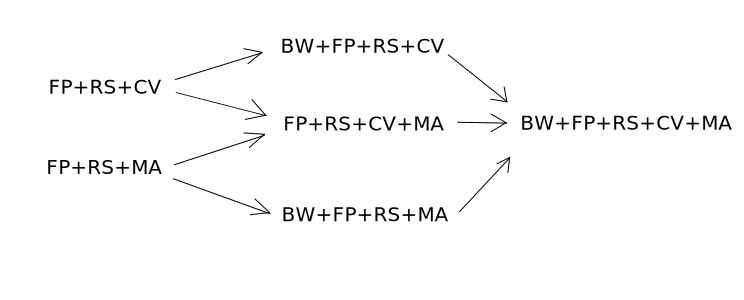
\includegraphics[width = \columnwidth]{figs/np-hierarchy}
\end{figure}



\subsection{Introduction to 3D Perfect Matching}

We start by introducing the NP-complete problem of 3D Perfect Matching
that will serve as problem we reduce from in both proofs. This problem
can be seen as a generalization of bipartite matchings to 3-uniform
hypergraphs, henceforth called $\TDM$.~\cite{3dmatch}

$\TDM$ is defined as follows. We are given three finite and disjoint
sets $X$, $Y$, and $Z$ of cardinality $k$, as well as a subset of triples $T\subset
X \times Y \times Z$.  Set $M \subseteq T$ is a 3-dimensional matching
if and only if, for any two distinct triples $(x_1, y_1, z_1) \in M$
and $(x_2, y_2, z_2) \in M$, it holds that $x_1\neq x_2$, $y_1\neq
y_2$, and $z_1\neq z_2$. Our goal is to decide if we can construct
such $M \subseteq T$ that is perfect, which means that it covers all
elements of $X \times Y \times Z$.

TODO: cite Karp on result of NP-completeness
TODO: image like this: \url{https://upload.wikimedia.org/wikipedia/commons/thumb/5/50/3-dimensional-matching.svg/240px-3-dimensional-matching.svg.png}

\subsection{Multi-Assignments are hard ($\FP+\RS+\MA$)}\label{ssec:fprsma}

Here we will present high-level ideas about encoding $\TDM$ as
 $\FP+\RS+\MA$ instance:

 \begin{itemize} \item For every element of universe $X\cup Y\cup
 Z$, we create chunk type. Processing every chunk corresponds to
 covering whole universe.

 \item We will encode each tripple as $3$ leaves that are close to
 eachother. We place chunk replicas that correspond to elements of the
 tripple.

 \item Placement of VMs will correspond to choice of tripples. No
 matter in which leaf of the gadget the VM will spawn, we will take
 that tripple to solution. VM will process the chunk that it sits on
 top of, as well as chunks in other two leaves of the same gadget.
 
\item We will set threshold cost in such way that no VM process
any chunk outside of the gadget that VM sits in.
\end{itemize}

\textbf{Construction.}
Given an instance $I$ of $\TDM$, we construct an instance $I'$ of
$\FP+\RS+\MA$ as follows:
\begin{itemize}
\item (tree construction) We create a tree consisting of root vertex, and for each tripple
we create a gadget that we attach as direct child of the root. Each
gadget consists of four vertices, one being inner node and three
leaves (see figure below).
\item (chunks and chunk replicas) For each element in $X$, $Y$ and $Z$ we create chunk type
($3 \cdot k$ in total). For each tripple we create $3$ replicas of
chunks that correspond to elements of universe and we place those
replicas in leaves of corresponding gadget
\item (other properties) We set number of VMs to spawn to $k$; we set
$\CostTrans=1$; we set number of slots in each VM to $m=3$; we set
$\Thr=2 \cdot 2 \cdot k$
\end{itemize}

FIXME: The construction is illustrated in Figure~\ref{fig:fprsma}.

\textbf{Correctness.}
We can now show the computational hardness.
\begin{theorem}
$\FP+\RS+\MA$ is NP-hard.
\end{theorem}
\begin{proof}
Let $I$ be an instance of $\TDM$ and let $I'$ be an instance of
$\FP+\RS+\MA$ constructed as described above.
We prove that $I'$ has solution of cost $\leq \Thr$ if ($\Rightarrow$) and only if
($\Leftarrow$)
$I$ has a matching of size $k$.

($\Rightarrow$) Let us take a solution to $\TDM$. We spawn VM in every
gadget that corresponds to chosen triples. We match every chunk in a
gadget to machine in this gadget (only for chosen ones). Solution has
cost exactly $\Thr$.

($\Leftarrow$) Let's take solution to $VC$ instance of cost $\leq \Thr$. We
chose triples that correspond to gadgets where were VMs. Everything
was processed, therefore every element of X,Y and Z is matched.
\end{proof}


\subsection{Inter-connects are hard ($\FP+\RS+\CC$) (reduction from 3D Perfect Matching)}\label{ssec:fprscc}


Next, we prove that the joint optimization of node placement and replica selection
is NP-hard if an inter-connect has to be established between virtual machines.
In our terminology, this is the $\FP+\RS+\CC$ problem.


\textbf{Construction.}
Given an instance of $\TDM$, we construct an instance of a
$\FP+\RS+\CC$ problem as follows. For each element
in the universe $X \cup Y \cup Z$, we construct a chunk; and for each
tripple $T_i$, we construct a gadget that contains
three replicas of chunks corresponding to the elements in the subset (those have 2 hops distance to eachother).
We connect the gadgets to the root, separating nodes from different tripples by 4 hops.

Concretely, let $I$ be an instance of $\TDM$. We will create an instance $I'$
for $\FP+\RS+\CC$ as follows:
\begin{itemize}
\item We set the access cost $\CostTrans$ to a chunk replica to a high value $W$. This will force
nodes to be collocated with the replica.
(For now, we can assume that $W=\infty$; a lower and sufficient bound will be given
in the appendix.)
\item The communication cost in the inter-connect is set to $\CostCom = 1$.
\item The number of nodes (virtual machines) is $\Vms = 3 \cdot k$. TODO: check again
\item We use a threshold $\Thr =  3 \cdot k + 3 \cdot 3 \cdot 2 \cdot (k - 1)$. TODO: check again
\end{itemize}

We construct a height-2 substrate tree
as follows. For each $T_i$ we construct a gadget
consisting of an inner node (a router) and three leaves. Every gadget
contains three chunks, corresponding to the elements of $T_i$.

FIXME: The construction is illustrated in Figure~\ref{fig:fprscc}.

\textbf{Proof of correctness.}
Intuitively, in order to minimize embedding costs,
nodes should be placed on near-by replicas. We use the following
helper lemma.
\begin{lemma}\label{lemma:helper}
In every valid solution $\Sol$ of $I'$ of cost $\leq \Thr$, each gadget
falls in one of two categories:
$k$ gadgets have exactly
$3$ nodes, and $n-k$ gadgets remain empty.
\end{lemma}
\begin{proof}
TODO: use exact cover property here to reason about feasibility

Since $W=\infty$, nodes will always be placed
directly on chunks (the access network cost is zero).
Moreover, since
$\Sol$ is valid, $3 \cdot k$ nodes are mapped
directly to the different chunk locations.
Now, consider any pair of nodes communicating over the
inter-connect; due to our construction, the communication cost
for each such pair is either
2 hops (if they belong to the same gadget) or 4 hops (if they belong
to different gadgets).
The lemma then follows from the observation that $\Thr$
is chosen such that it is never possible to distribute nodes
among more than $k$ gadgets, and that it is always strictly better to
have exactly 0 or 3 nodes per gadget, than any alternative distribution.
\end{proof}

\begin{theorem}
$\FP+\RS+\CC$ is NP-hard.
\end{theorem}
\begin{proof}
Let $I$ be an instance of $\TDM$ and let $I'$ be an instance of
$\FP+\RS+\CC$ constructed as described above.
We prove that $I'$ has solution of cost $\leq \Thr$ if ($\Rightarrow$) and only if
($\Leftarrow$)
$I$ has a solution.

($\Rightarrow$) In order to compute a solution
for $I'$ given a solution for $I$, we proceed as follows.
Given a covering set of tripples $S = \{T_1, T_2, \ldots, T_k\}$, we place three nodes in each gadget that
corresponds to every tripple of $S$. Chunks are matched to VMs that sit on top of them.

The solution has the following cost:
(1) the communication cost inside a gadget is $2 \cdot {3 \choose 2}$,
  as every pair contributes two hops;
  (2) the communication cost from each gadget to all other gadgets is $4
  \cdot 3 \cdot 3 \cdot (k - 1) / 2$, where the factor $2$ is
  for the
  communication over $4$ hops, the factor $3$
  corresponds to the number of nodes per gadget, and
  $3 \cdot (k-1)$ is the number of nodes in remote gadgets;
  as we count each pair twice, we need to divide by two in the end.
Summing up over all $k$ gadgets, we get exactly $\Thr$.

($\Leftarrow$) Given a solution for $I'$,
we can exploit Lemma~\ref{lemma:helper} to construct a solution for $I$.
We know that in any solution of cost at most $\Thr$,
$k$ gadgets contain exactly 3 nodes. These gadgets correspond to a valid
3D Perfect Matching of size $k$: every
chunk and hence element in the $X \cup Y \cup Z$, is matched.
\end{proof}




%%%%%%%%%%%%%%%%%%%%%%%%%%%%%%%%%%%%%
\section{Related Work}\label{sec:relwork}

Our work is motivated by the resource allocation and computational model of
batch-processing cloud applications, such as MapReduce.
These applications
generate large amounts of network traffic, and a considerable
fraction of the runtime is due to network acti\-vi\-ty.~\cite{talk-about,amazonbw,orchestra}.
Accordingly, systems have been proposed which provide
a provable network performance by making explicit bandwidth reservations
between the virtual machines or compute units, either relative~\cite{seawall,faircloud,elasticswitch}
or absolute~\cite{secondnet,oktopus, proteus, drl, gatekeeper}.

The need to take into account both node as well as link resources motivates
the design of virtual networks, and the question of how to efficiently embed virtual networks
has been studied intensively, also from an algorithmic perspective.
For a good survey on network virtualization and in particular virtual network embeddings,
we refer the reader to~\cite{boutaba-survey} and~\cite{fischer-survey}.

The most popular abstraction for batch-processing applications is the virtual cluster,
introduced in the Oktopus paper~\cite{oktopus}, and later studied by many other researchers~\cite{proteus}.
Many heuristics have been developed to compute ``good'' embeddings of virtual clusters, in the sense that
they result in small footprints (minimal bandwidth reservation costs).

However, the virtual network embedding problem has not only been studied for virtual clusters,
but also for more general graphs (motivated by wide-area networks). In contrast to the classic VPN
graph embedding problems~\cite{gupta2001provisioning,Goyal2008},
in these models, also the embedding endpoints are flexible and subject to optimization.
In this respect, the problem can also be seen as a generalization of the classic NP-hard Minimum Linear Arrangement problem which asks for the
embedding of guest graphs on a simple line topology.~\cite{mla,mla-survey,mla-feige}
Indeed, many problem variants are NP-hard and much research so far has focused on heuristics~\cite{ammar,zhu06,simannealing,turner}
or mixed integer programs~\cite{infocom2009,ucc12mip}.

However, to the best of our knowledge, we are the first to provide an algorithmic
study of the cloud application embedding problem which also takes into account
data locality as well as the possibility to select replicas. As we have shown in this paper,
the resulting problems can be seen as interesting new variants of several classic optimization
problems, such as hitting sets, matchings and 3-dimensional matchings~\cite{3SC-hard} as well as cover and flow problems.~\cite{korte2002combinatorial}


%%%%%%%%%%%%%%%%%%%%%%%%%%%%%%%%%%%%%
\section{Summary and Conclusion}\label{sec:conclusion}

This paper investigated two fundamental new dimensions of virtual cluster
embedding problems: data locality and replica selection. We pursued
an algorithmic approach and decomposed the problem into fundamental aspects,
namely $\BW$, $\CC$, $\RS$, $\MA$ and $\FP$. Our results are summarized in
Figure~\ref{fig:summary}.
In particular, we have shown that
at the heart of our problem lie interesting new variants of classic
optimization problems related to matchings and flows. Interestingly, despite the
numerous
flexibilities, many problem instances can actually be solved in polynomial time.
On the negative side, we have also shown that there exist computationally hard
problems even in uncapacitated networks. In particular,
we have shown that several embeddings problems are NP-hard already in two-level fat-trees (practically speaking:
problems inside a single \emph{pod}), and even if the the number of replicas is bounded by two.


\begin{figure}[t]
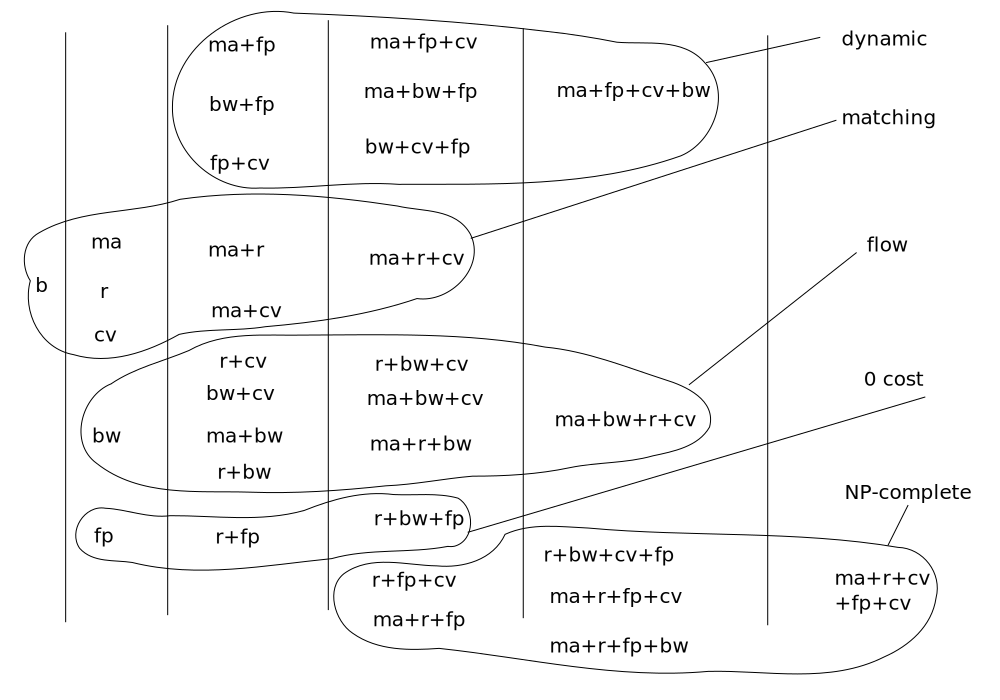
\includegraphics[width = \columnwidth]{figs/summary}
\caption{Summary of results. As this paper only presented algorithms for the most
difficult problems and, respectively, proved NP-hardness of the simplest
problems, several additional results are simple implications (indicated by arrows).}
\label{fig:summary}
\end{figure}


Our paper provides an almost complete overview of what can and cannot be
computed optimally in our setting, and may of interest both to the algorithm
and the networking community. However, our work also opens several interesting
questions for future research, for instance, regarding randomized algorithms
or approximation algorithms. A concrete and particularly interesting open
question is whether FIXME.



%%%%%%%%%%%%%%%%%%%%%%%%%%%%%%%%%%%%%
%\bibliographystyle{alpha}
\bibliographystyle{abbrv}
\bibliography{references}

%%%%%%%%%%%%%%%%%%%%%%%%%%%%%%%%%%%%%
\begin{appendix}


\section{Bandwidth Lemma}

The following lemma is useful in our NP-hardness proofs.

\begin{lemma}[Bandwidth Lemma]\label{lem:bandwidth-lemma}
  Let $c$ and $v > 4$ be two arbitrary positive integers. Let $a_1, a_2, \ldots,
  a_v$ be a sequence of $v$ integers which adds up to $c \cdot v$. Also, for
  each $i$ we have $a_i \leq 2 \cdot c$. Then it holds that if
  $$ \forall_i a_i \cdot (c \cdot v - a_i) \leq c \cdot (c \cdot v -
  c), $$
\noindent  then for each $i$, $a_i = c$.
\end{lemma}
\begin{proof}
For the sake of contradiction, let us assume that there exists an index $k$ such that
$a_k \neq c$. Then we can distinguish between two cases:
either $a_k<c$ or
$a_k>c$.

\textbf{Case $a_k<c$:} If there exists a $k$ with $a_k<c$,
due to the fact that the sequence sum adds up to $c \cdot v$,
there must also exist a $k'$ such that $a_{k'}<c$ (by a simple
pigeon hole principle). Thus, this case can
also be reduced to the second case (\textbf{Case $a_k>c$}) proved
next

\textbf{Case $a_k>c$:} Since it also holds that $a_k < 2c$,
$a_k$ must be of the form $c + x$ for $x \in [1, \ldots, c]$.
Let us consider the (bandwidth) inequality:
$$ (c + x) \cdot (c \cdot v - c - x) \leq c \cdot (c \cdot v - x) $$

This can be transformed to:

$$ 0 \leq x(x - (c \cdot (v - 2))) $$

The equation holds for $x \leq 0$ or $x \geq c \cdot (v - 2)$,
and no
positive $x \leq c$ can satisfy this inequality for $v > 4$. Contradiction.
\end{proof}


\section{Capacities are hard ($\RS+\FP+\BW$)}

We prove that $\RS+\FP+\BW$ is NP-hard by reduction from the Boolean Satisfiability Problem ($\SAT$).
Since $\SAT$ is a decision
problem, we transform $\RS+\FP+\BW$ into a decision problem too, by
introducing a cost threshold $\Thr$.

Let's first recall that the $\SAT$ problem asks whether a positive valuation exists
for a formula $\Formula$ with $\clauses$ clauses and $\variables$ variables.
In the following, we will only focus on $\SAT$ instances of at least four variables;
this problem remains NP-hard.

\textbf{Construction.}
Given any formula $\Formula$ in Conjunctive Normal Form (CNF) with at least four variables, we produce
a $\RS+\FP+\BW$ instance as follows. First, we construct a substrate tree $\Tree_{\Formula}$, consisting of
a root and separate gadgets for each variable of $\Formula$, each of which
is a child of the root.
The gadget of variable $v$ has a root, $\aroot(v)$, and two children:
$\positive(v)$ and $\negative(v)$. Vertex $\positive(v)$ has $\clauses$
many children $v_1, v_2, \ldots, v_{\clauses}$, and vertex $\negative(v)$ has
$\clauses$ many children $\neg v_1, \neg v_2, \dots, v_{\clauses}$. Every
gadget has the same structure: the same height and the same number of
leaves. By default, we will set the available bandwidth to be the
same everywhere, in every gadget; differences will be shown when we
will place chunks.

We set the number of virtual machines to $n = \clauses \cdot \variables$.
Moreover, we define the inter-connect communication cost to be $1$,
and the access cost to be a sufficiently large constant $W$,
such that nodes must always be collocated with chunks.
(For a concrete value, use $W=$TODO).


We set the following bandwidth capacities in the substrate. There are three
levels of edges in the substrate tree $\Tree_{\Formula}$ given by formula
$\Formula$: \emph{top}, \emph{middle} and \emph{bottom}.
We do not consider any capacities at the \emph{bottom} and \emph{middle} levels.
At a top-level edge, we set the bandwidth to $\clauses \cdot (\variables -
\clauses)$.

We set the number of chunks to be equal to the number of clauses, $\ChunkTypes =
\clauses$. To finish our construction, we place data chunks at
leaves, as follows: for the $i$-th clause we
construct as many replicas of chunk $\achunk_i$ as there are literals in the
clause. For each literal $\ell$ (of the form $v$ or $\neg v$) that satisfies clause $i$ we place
replica of chunk $\achunk_i$ in leaf labeled $\achunk_{\ell_i}$.

The threshold $\Thr$ is given by the
communication cost among nodes in
a certain solution to our instance. This solution is constructed by embedding
nodes at all leaves of $\positive(v)$ and none at leaves
$\negative(v)$, for every gadget for variable $v$. Please note that $\Thr$
computed such way do not contain transportation cost. TODO: calculate
$\Thr$.

\textbf{Proof of correctness of construction.}
With our construction completed, we need to prove that it indeed
decides $\SAT$. We set the capacities such that in every gadget,
at most $\clauses$ nodes can be spawned, where $\clauses$
is the number of clauses of $\Formula$.
We can apply the Bandwidth Lemma (Lemma~\ref{lem:bandwidth-lemma}) as follows:
We interpret $a_i$ as the
number of nodes that are embedded in the $i$-th gadget; we set $c=\clauses$
to be the number
of clauses and $v=\variables$ to be the number of variables.
The LHS of the inequality of Lemma~\ref{lem:bandwidth-lemma}
is a formula for the communication cost of nodes inside the $i$-th
gadget to nodes outside the gadget. The RHS of the inequality is the
bandwidth constraint for the gadget. This implies that
any feasible solution must embed exactly $c$ nodes in every gadget.


\begin{theorem}
The problem $\RS+\FP+\BW+\CC$ is NP-hard.
\end{theorem}
\begin{proof}
We will prove that formula $\Formula$ is satisfiable iff $\RS+\FP+\BW+\CC$ has
solution of cost $\leq \Thr$.

($\Rightarrow$) Let's take any valuation $\Val$ that satisfies $\Formula$.
We will construct a solution to $\RS+\FP+\BW$ using $\Val$ in the following way.
For each variable $v$ in $\Formula$, we embed $\clauses$ many virtual machines
at the  leaves of the gadget of $v$. We need to choose $\clauses$ out of
$2 \cdot \clauses$ leaves to embed nodes. If $\Val(v) = 1$, we embed
nodes at the leaves
of $\positive(v)$, else we embed all nodes at leaves $\negative(v)$.
The solution constructed this way has cost exactly
$\Thr$, because the nodes are evenly split among gadgets, and nodes are not
distributed across $\positive(v)$ and $\negative(v)$ subtrees.

We calculate the matching of chunks to VMs by matching every chunk to
VM that sits on top of first chunk replica. This solution is feasible
(every chunk type is processed) basically
because given valuation satisfied the $\Phi$.

Now we will show that this solution has cost $\Thr$.
Due to the Bandwidth Lemma (Lemma~\ref{lem:bandwidth-lemma}),
we only have to consider the communication cost.

($\Leftarrow$) Let's take any solution to $\RS+\FP+\BW$ constructed based on $\Formula$ of cost $\leq \Thr$.
We will construct a positive valuation $\Val$ by considering the nodes in
the solution to $\RS+\FP+\BW$.

We make the following observations. In every solution of cost
$\leq \Thr$, every gadget has exactly $\clauses$ many nodes
at its leaves. This is due to the Bandwidth Lemma. Also, inside
every gadget either all nodes are in the $\positive(v)$ subtree
of variable $v$, or in the $\negative(v)$ subtree. This is true
because the cost of a solution where at least one gadget has nodes
distributed across subtrees is
always greater than $\Thr$.

TODO Maciek: prove it more formally. First, define semi-feasible solution. Let's take any $p,q$ being the number of nodes
spawned in left and right subtree. Then we say that we can improve the
solution by moving all $q$ to where $p$s lie and we have cheaper solution.

Now we can construct our valuation $\Val$, as follows
(for each variable $v$ in $\Formula$):
If $v_1$ hosts a node then $\Val(v) = \top$,
otherwise $\Val(v) = \bot$.

The valuation $\Val$ satisfies all clauses, and hence $\Formula$,
as the solution to $\RS+\FP+\BW$ covers all chunks. To see this,
consider the leaf handling any given clause chunk;
it is a witness that the corresponding clause is true.
\end{proof}

\subsection{Two replicas are hard ($\FP+\RS(2)+\BW+\CC$)}\label{ssec:two}

Our results so far indicate that dealing with replication can be challenging.
However, all our hardness proofs concerned scenarios with three replicas,
which raises the question whether the problems can be solved in polynomial time
with a replication factor of two only. (Similarly to, say, the $\ZSAT$ problem
which is tractable in contrast to $\TSAT$.)

In the following, we show that this is not the case: the problem remains
NP-hard, at least in the capacitated network.

The proof is by reduction from $\TSAT$. Given a formula $\Formula$ in
conjunctive normal form, consisting of $\clauses$ clauses and $\vars$ variables, we construct a problem instance and substrate tree
$T_{\Formula}$ using two types of gadgets: gadgets for variables and
gadgets for clauses. Nota bene:
unlike in the previous proofs, for every clause we will create three chunk types instead of just one.

\textbf{Construction.}
We distribute chunks among servers as follows. First,
similarly to the previous proofs with three replicas, we put clause chunks in
variable gadgets; however, now we place distinct chunks instead of
three copies of the same chunk. Second, we place three chunks that
correspond to clauses in all three leaves of their clause gadgets.
Thus, in total, $6 \cdot \clauses$ variable chunks are mapped.
We will consider a setting where $cv + 2\clauses$ nodes need to be mapped. Our intention is that in
every variable gadget, there will be $\clauses$ nodes,
 and in every of clause
gadgets there will be two nodes.

The available bandwidth of the top edge of the gadget of each variable $v$ is set to
$\capa(v) = 3  \cdot  3  \cdot  (3  \cdot  (\vars - 1) + 2  \cdot  \clauses) $.
The first factor is the tree distance which is 6 divided by 2 (as
we count each pair twice). The second factor is
the number of nodes to be placed in every variable gadget.
So the first term of the
sum is three times the number of outer variable gadgets,
and the second term is the
number of nodes in each of the $\clauses$ clause gadgets.

The available bandwidth for the top edge of each clause gadget is set to
$\capa(\clauses) = 3  \cdot  2  \cdot  (2  \cdot  (\clauses - 1) + 3  \cdot  \vars) $.

FIXME: The construction is illustrated in Figure~\ref{fig:two}.


\textbf{Proof of correctness.}
We first prove the following helper lemma.
\begin{lemma}
Every valid solution to $\FP+\RS(2)+\BW+\CC$
with cost at most $\Thr$ has the property that
there are exactly $\clauses$ nodes in each of the $\vars$ variable gadgets
and exactly two nodes in each of the $\clauses$ clause gadgets.
\end{lemma}
\begin{proof}
The claim is due to the bandwidth constraints. We have to take into
consideration the following communication paths:
communication to clause gadgets and
communication to
other variable gadgets.
In every valid solution of cost at most $\Thr$ we have exactly
$\clauses$ nodes in each variable gadget and two nodes in each clause gadget.
\end{proof}

\begin{theorem}
$\FP+\RS(2)+\BW+\CC$ is NP-hard.
\end{theorem}
\begin{proof}
We show that $\FP+\RS(2)+\BW+\CC$ has a solution of cost $\leq
  \Thr$ if and only if $\Formula\in \TSAT$ is satisfiable.

($\Rightarrow$) If we have a positive valuation of $\Formula$, we fill variable gadgets with nodes like in
the proofs before. Then we fill $2 \cdot \clauses$ nodes as follows:
\begin{itemize}
\item If the first literal satisfies the clause, we map two nodes in the second and
third leaf of the corresponding clause gadget.
\item If the first literal does not satisfy the clause, we map two nodes to the first
and second leaf of the clause gadget.
\end{itemize}

TODO: chunk assignment should be based on valuation!

We then assign chunks to nodes as follows:
\begin{itemize}
\item Chunk $\achunk_i^1$ is matched to the node which is located in a variable gadget; there
must be one, as the valuation satisfies the formula.
\item Chunks $\achunk_i^2$ and $\achunk_i^3$ are matched to nodes which are
located in clause
gadgets; there exist minimal-cost solutions where nodes sit there.
\end{itemize}

Thus, we have produced a feasible solution of cost $\Thr$, as there are no
access and inter-connect costs.

($\Leftarrow$)
Let's take any solution $\Sol$ to $\FP+\RS(2)+\BW$ of cost $\leq \Thr$.
Then we can compute a positive valuation by setting each variable $v$
as follows:
$\Val(v)= \top$ iff there lies VM on first leaf on positive side of $v$ gadget in $\Sol$,
and $\Val(v)=\bot$ otherwise.

%$\Val(v)$ =
%\begin{cases}
%\top & \mbox{iff there lies VM on first leaf on positive side of $v$ gadget in $\Sol$}\\
%\bot & \mbox{otherwise}
%\end{cases}

The theorem now follows from the following two additional lemmas.
\begin{lemma}
For every clause there exists a node in a variable gadget that processes one of
  three chunks that correspond to that clause.
\end{lemma}
\begin{proof}
 Each of the three chunks that correspond to every clause,
 is assigned a collocated node.
 At least one of those three nodes is not idle in a variable gadget;
otherwise, those two VMs in clause gadgets would not suffice in
satisfying all chunk types.
\end{proof}

Observation. It might happen that in $\Sol$, two nodes in
clause variables are idle, and three nodes in variable gadgets are
processing those $3$ chunk types. In this case, we
arbitrary nodes can be taken in the rest
of the proof.

\begin{lemma}
$\Val$ satisfies $\Formula$.
\end{lemma}
\begin{proof}
Let us consider the matching $M$ of $\Sol$, and let us consider an arbitrary clause of
$\Formula$ as well as its $3$ chunk types: $\achunk_i^1, \achunk_i^2, \achunk_i^3$.
We will refer to the nodes corresponding to them
by $v_i^1, v_i^2, v_i^3$; two of them lie in clause gadgets.
Take the chunk type that was processed in variable
gadgets and look at where it was processed.
In our valuation $\Val$, we set the literal of the node leaf to
$\top$; therefore the clause is satisfied.
\end{proof}
\end{proof}

\subsection{Images}

\begin{figure}[htbp]
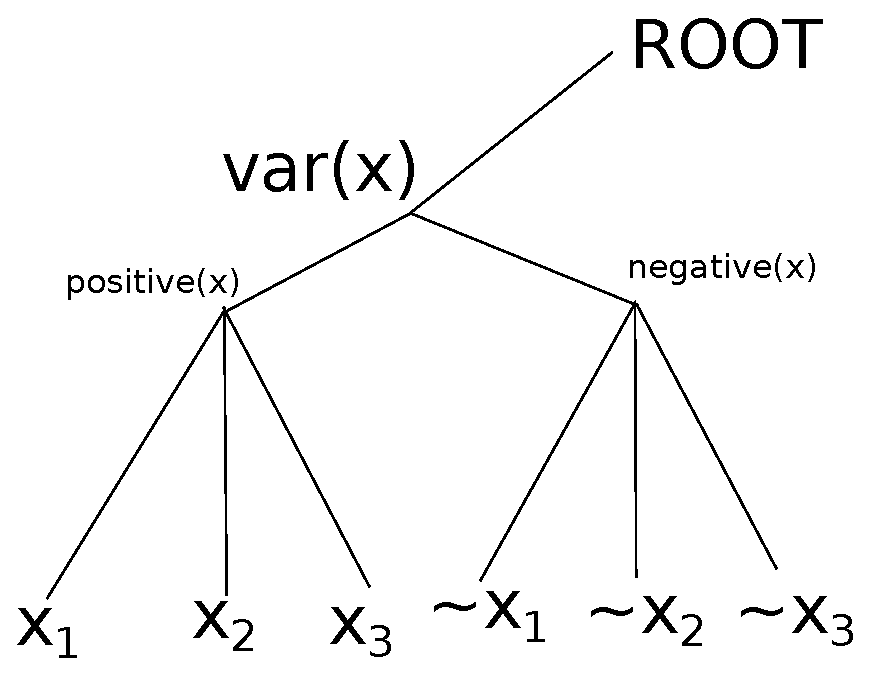
\includegraphics[width = \columnwidth]{figs/gadget-no-bw}
\end{figure}


\begin{figure}[htbp]
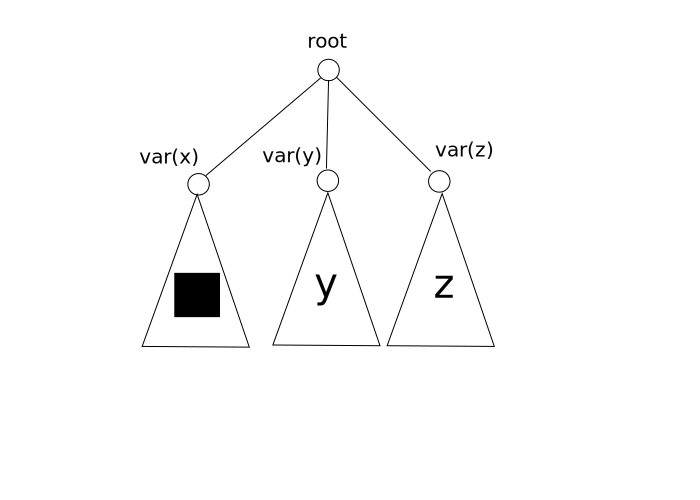
\includegraphics[width = \columnwidth]{figs/vc-instance}
\end{figure}


\begin{figure}[htbp]
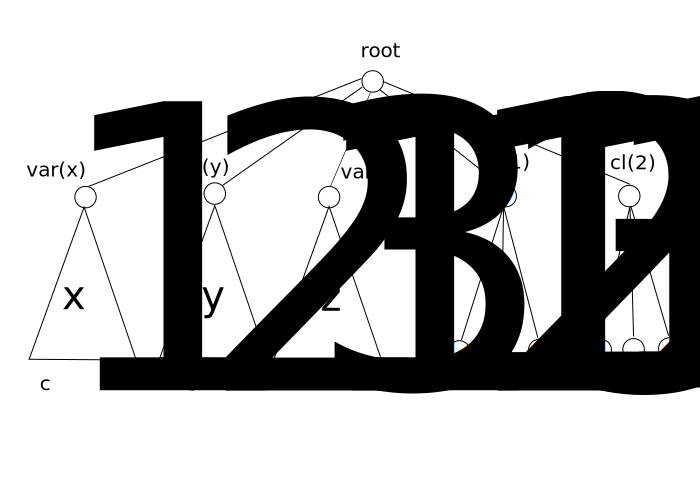
\includegraphics[width = \columnwidth]{figs/vc-instance-r2}
\end{figure}


\begin{figure}[htbp]
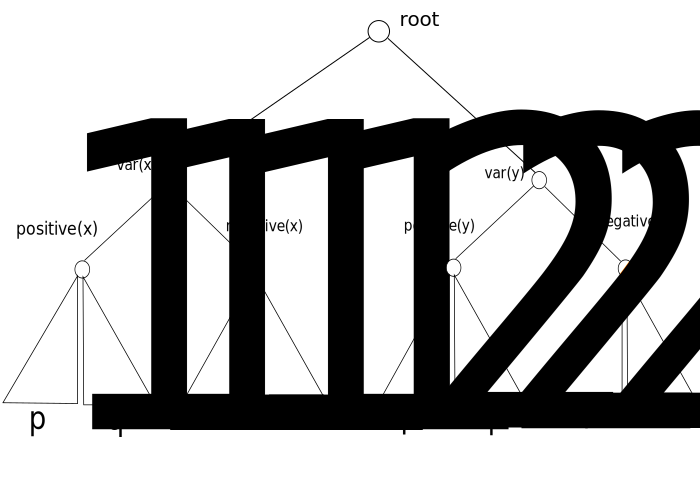
\includegraphics[width = \columnwidth]{figs/lemma-two-gadgets}
\end{figure}


\begin{figure}[htbp]
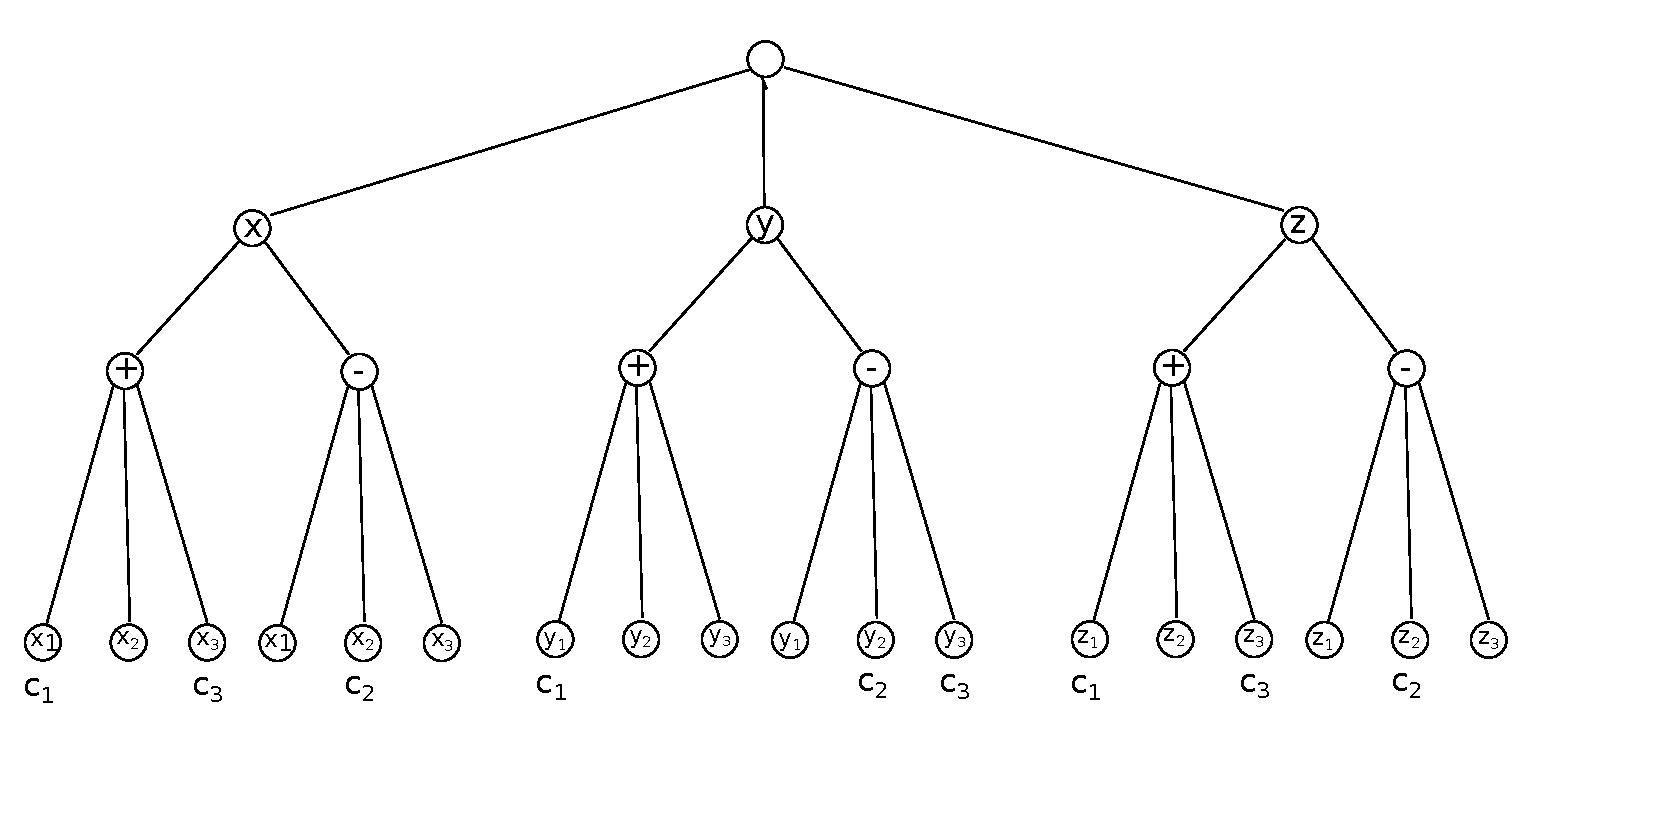
\includegraphics[width = \columnwidth]{figs/formula-example}
\end{figure}


\begin{figure}

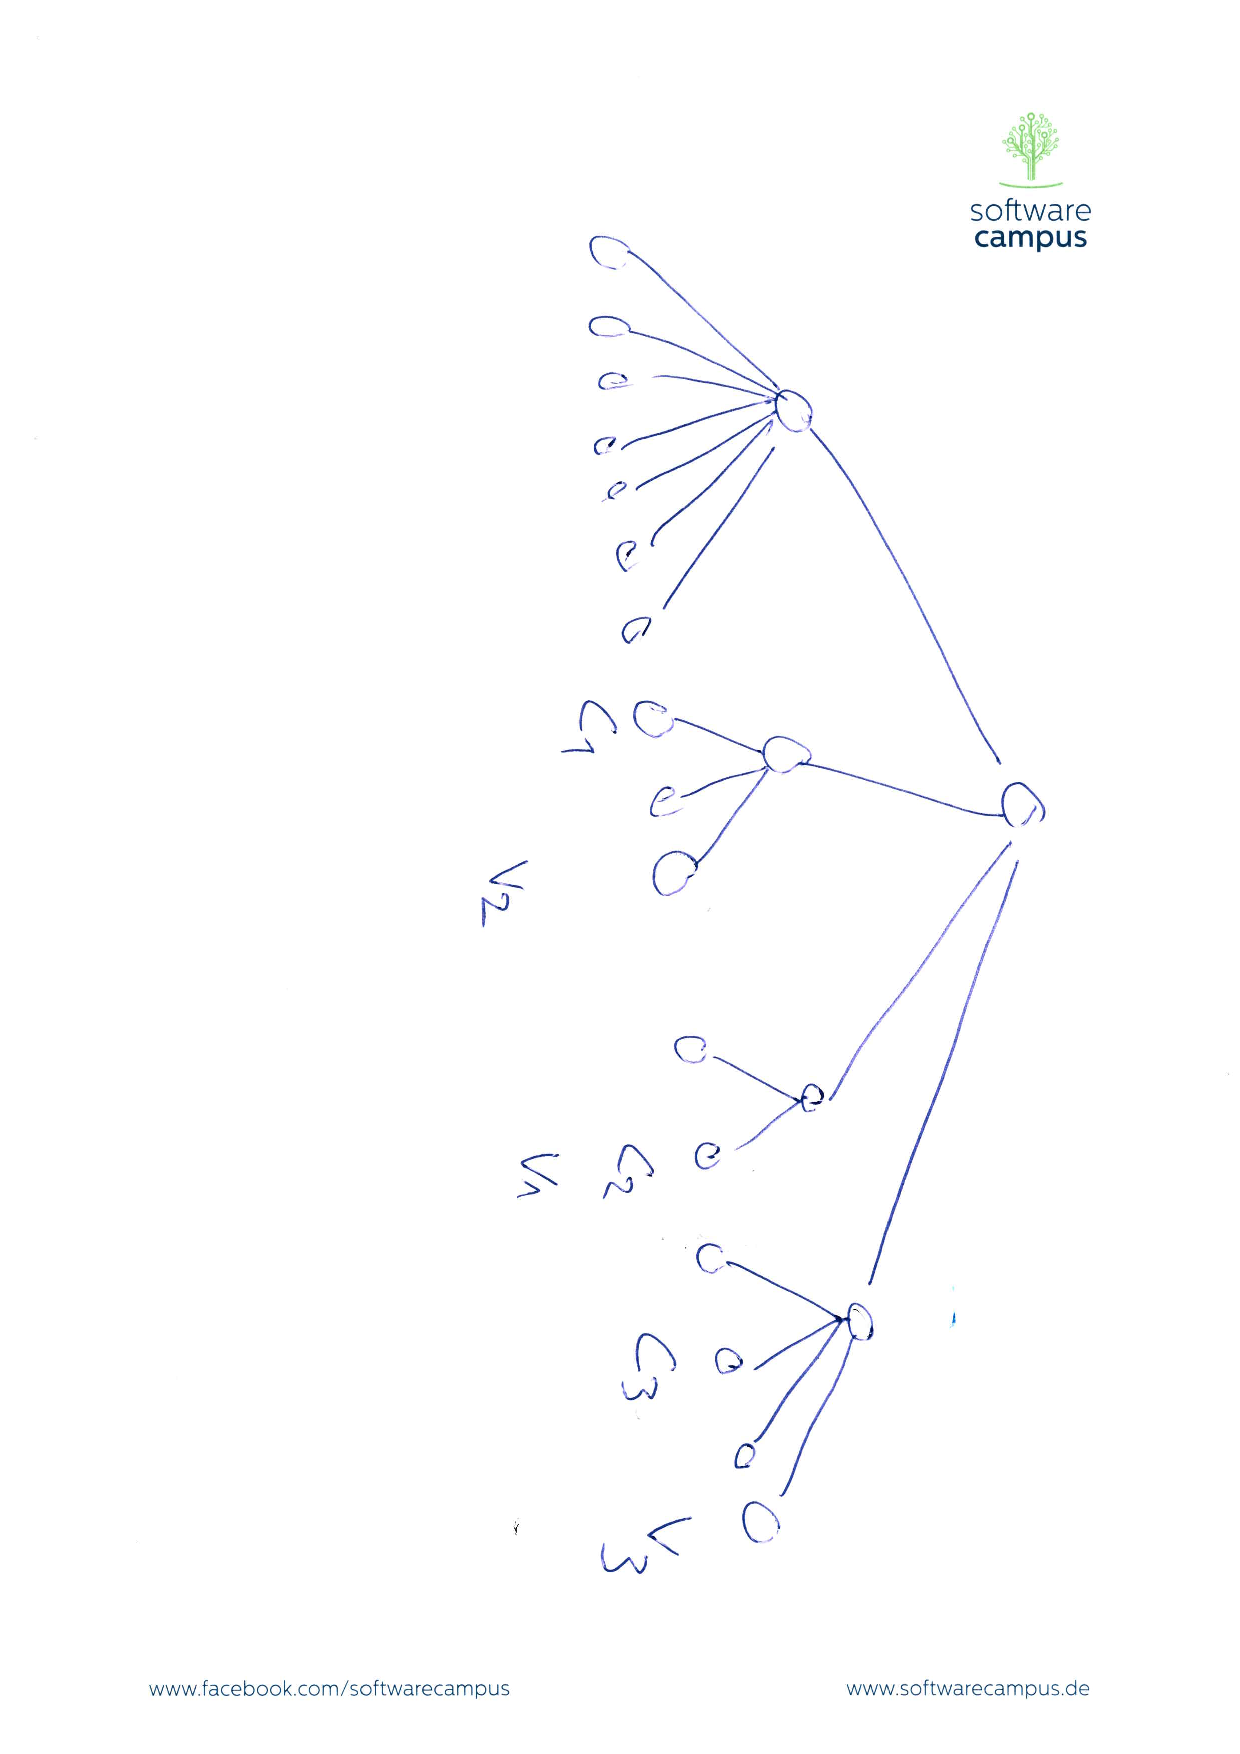
\includegraphics[angle=90,origin=c, height=7cm]{figs/model_fig_skteches/basic_problem}
\caption{basic problem}
\label{fig:basic_problem}
\end{figure}
\begin{figure}

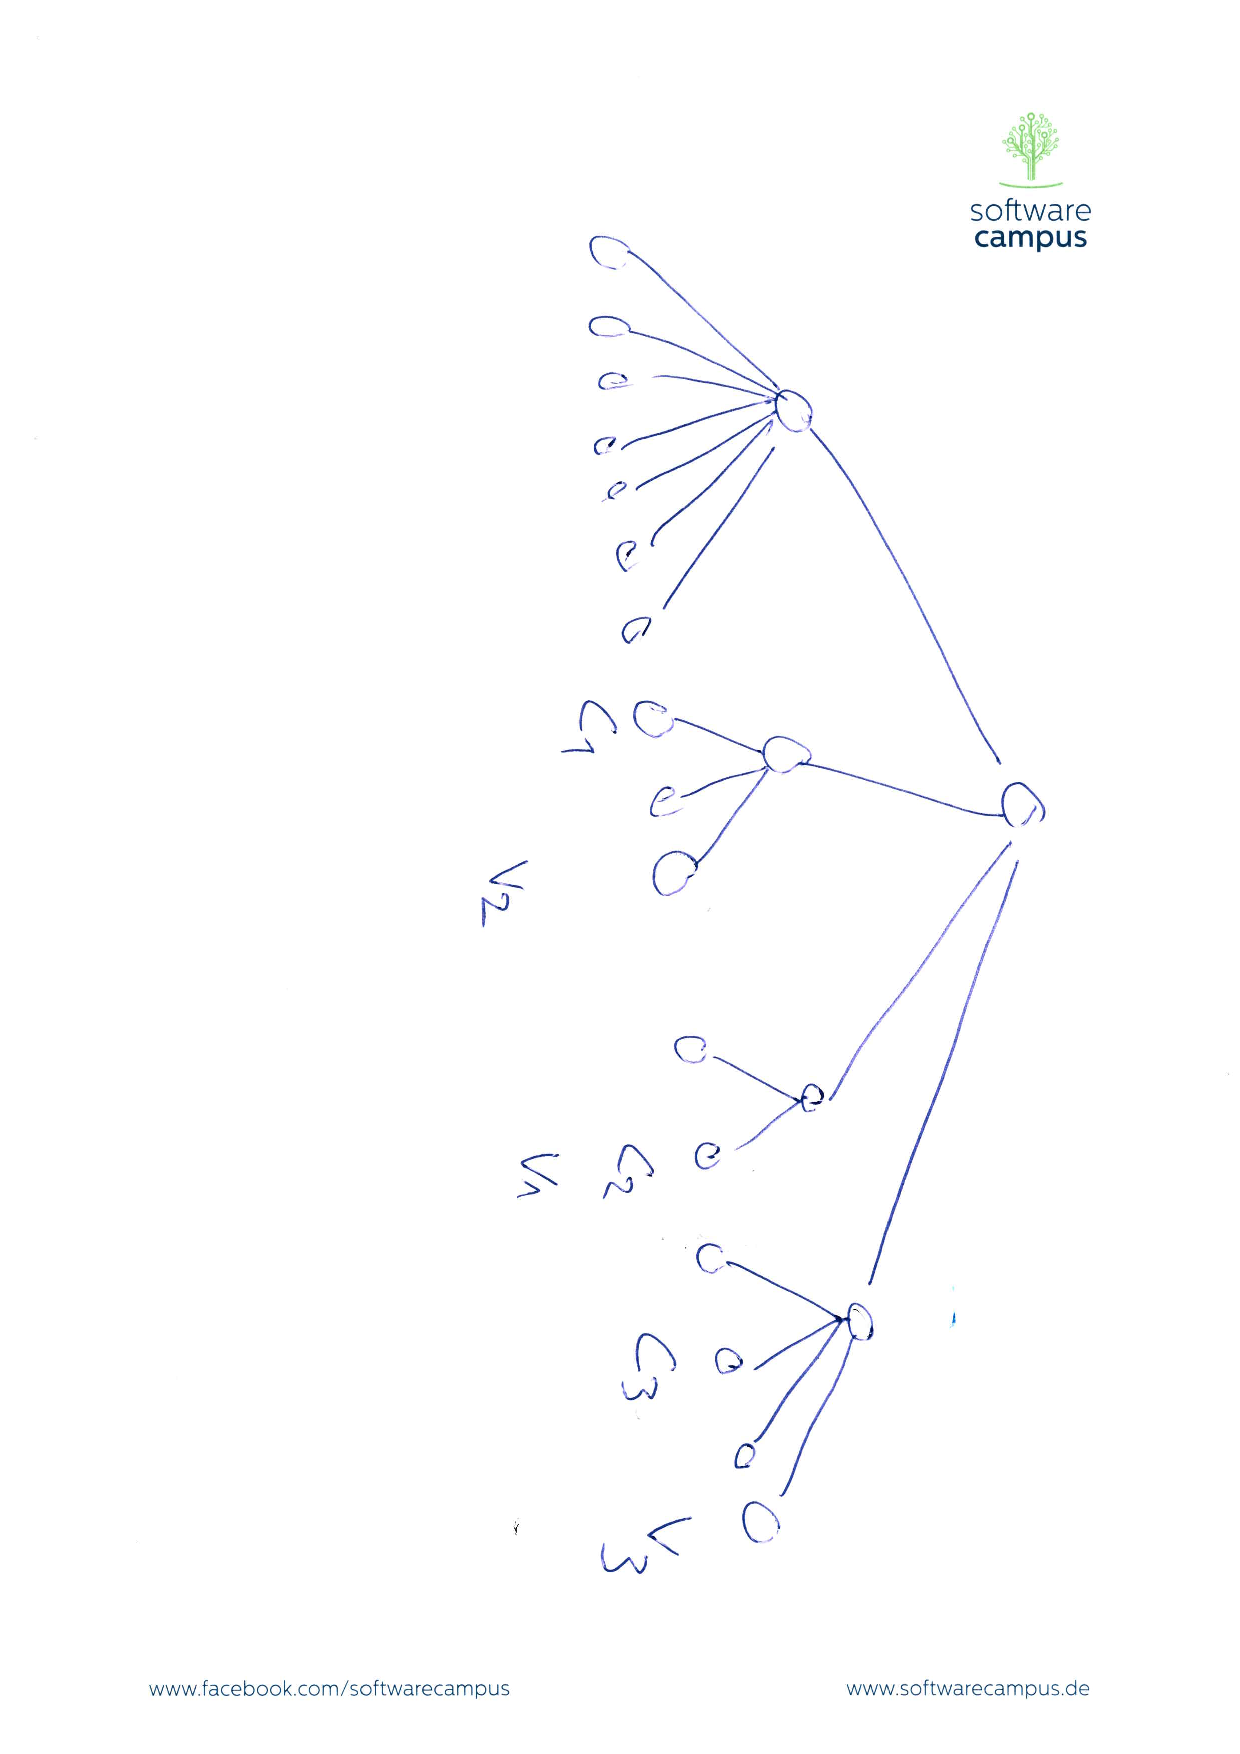
\includegraphics[angle=90,origin=c, height=7cm]{figs/model_fig_skteches/basic_problem}
\caption{solution for basic problem (green is pathes for transfer)}
\end{figure}

\section{Model}

This section describes our model. We will start by describing a simplistic
version of our model, and continue to introduce new properties until we reach
the full model.

\subsection{Symbols}

This is a dummy section to introduce the symbols used later...

\begin{description}
 \item [$\Tree$] the substrate tree with $\Tree = (\SubstrateNodes , \SubstrateEdges)$
 \item [$\SubstrateNodes$]  a set of nodes: $\{\SubstrateNode_1, \dots ,
\SubstrateNode_{|\SubstrateNodes|}\}$
 \item [$\SubstrateEdges$] a set of edges : $\{\SubstrateEdge_1, \dots ,
 \SubstrateEdge_{|\SubstrateEdge|}\}$ with $\SubstrateEdge_1 =
(\SubstrateNode_i, \SubstrateNode_j)$
 \item [$\achunk_i$] A chunk of type $i$
 \item [$v_i$] The i-th $\VM$ of the request
 \item [$\VirtualNodes$] the set of virtual Nodes = $\{1,2,\dots,\VCSwitch\}$
 \item [$\VirtualEdges$] the set of virtual Edges, $e_{V1}$ connects $1 \in
\VirtualNodes$ with $\VCSwitch \in \VirtualNodes$.
 \item [$\hat f$] the maximal flow
 \item [$|\hat f|$] the value of the maximal flow


 \item [$\Bandwidth$] Bandwidth constraint of an edge
 \item [$\CostTrans$] cost of chunk transport
 \item [$\CostCom$] cost of chunk communication
 \item [$\Vms$] number of VMs to spawn
 \item [$\ChunkTypes$] number of chunk types placed in an instance
 \item [$\Formula$] a formula
 \item [$\Clauses$] set of clauses in a formula
 \item [$\NClauses$] number of clauses in a given formula
 \item [$\Vars$] set of variables in a given formula
 \item [$\NVars$] number of variables in a given formula
 \item [$\Thr$] threshold
 \item [$\VCB$] virtual cluster model with bandwith
 \item [$\VCNB$] virtual cluster model without bandwith
 \item [$\varx$] variable
 \item [$\positive$] positive subtree of a gadget
 \item [$\negative$] negative subtree of a gadget
 \item [$\SAT$] set of satisfiable boolean formulas in CNF
 \item [$\TSAT$] set of satisfiable boolean formulas in 3CNF
 \item [$\Val$] valuation
 \item [$\Sol$] soultion to VC instance

\end{description}



\subsection{The Basic Model}

\carlo{Section TODO: How many / which figures + order?}

In the basic version of $\Problem$ data in the form of multiple chunks is
located in an undirected host graph tree $\Tree = (\SubstrateNodes,
\SubstrateEdges)$. A chunk $\Chunk$ of the set of chunks $\Chunks =
\{\Chunk_1,\dots,\Chunk_{\ChunkTypes}\}$ can only be located at the leaves
$\Leaves = \{\Leaf_1,\dots,\Leaf_m\} \subset \SubstrateNodes$ of $\Tree$. We
denote the location of a chunk by $\ChunkLocation : \Chunks \rightarrow
\Leaves$. A cluster, consisting of a set of VMs $\VirtualNodes =
\{\VirtualNode_1,\dots,\VirtualNode_{\Vms}\}$, is allready embedded on the host
graph, and should process this data. The VMs are embedded on the
leaves of the tree, and we denote the location of the VMs by $\NodeMapping :
\VirtualNodes \rightarrow \Leaves$. We assume that $\Vms = \ChunkTypes$, each
VM $\VirtualNode_i$ can read the data of one chunk $\Chunk_j$, and the data of
each chunk $\Chunk_j \in \Chunks$ has to be processed. In order to process the
data from a chunk $\Chunk_j$ with the VM $\VirtualNode_i$ it has to be
transferred along a (potentially empty) path $\Path_j =
\{\SubstrateEdge_{j_1},\dots,\SubstrateEdge_{j_n}\} ~ \SubstrateEdge_{j_k} \in
\SubstrateEdges$ such that $\SubstrateEdge_{j_1} = (\ChunkLocation(\Chunk_j),
\SubstrateNode_x)$, $\SubstrateEdge_{j_k} = (\SubstrateNode_x,
\SubstrateNode_y) \rightarrow \SubstrateEdge_{j_{k+1}} = (\SubstrateNode_y ,
\SubstrateNode_z)$, and $\SubstrateEdge_n = (\SubstrateNode_y,
\NodeMapping(\VirtualNode_i))$.  For the sake of simplicity we assume that
transferring a chunk over a link in the host graph inflicts bandwidth cost of
$\CostTrans$ on this link. \carlo{NEW: We refer to the sum of all bandwidth
costs for the transport of specific chunks to vms by the function
$\CostPerChunk : \Chunks \cup \VirtualNodes \rightarrow \mathbb{R}$. Note, that
$\CostPerChunk(\Chunk_j) = \CostPerChunk(\VmChunkAssignment(\Chunk_j))$ and
$\CostPerChunk(\Chunk_j) = \Distance(\ChunkLocation(\Chunk_j),
\NodeMapping(\VmChunkAssignment(\Chunk_j))) \cdot \CostTrans$, where $\Distance
: \SubstrateNodes \times \SubstrateNodes \rightarrow \mathbb{N}$ denotes the
distance in number of hops of two nodes in the host graph.} The overall
objective of $\Problem$ is to find an
assignment of VMs to chunks $\VmChunkAssignment : \Chunks \rightarrow
\SubstrateNodes$, so that the overall costs $\sum_{j \in
\{1,\dots,\ChunkTypes\}} |\Path_j|$ are minimized.

Throughout this section we will introduce different properties, to extend this
basic model. These properties can (and will) be combined to form more
challenging instances of $\Problem$.

%\begin{figure}[htbp]
%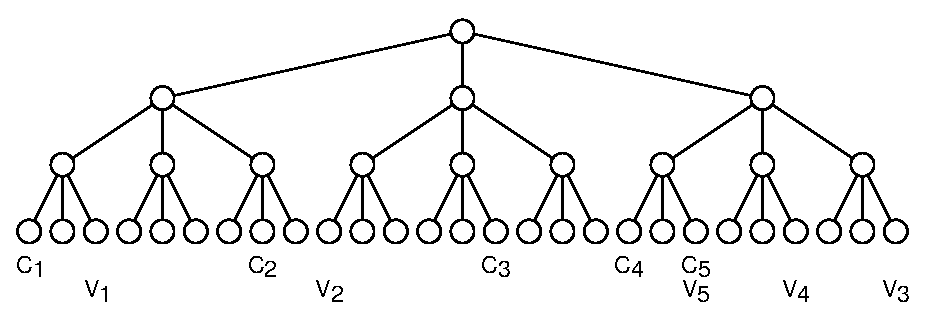
\includegraphics[width = \columnwidth]{figs/basic_scenario_3.eps}
%\caption{An example situation with 5 $\Chunk s$ and $\VM s$. Note that $c_5$
%and $v_5$ are on the same host.}
%\label{fig:model_clean}
%\end{figure}
%
%
%
%Figure~\ref{fig:model_clean} shows an example situation with $n = 5$. The goal
%of the $\Problem$  is to find an assignment of the $\VM s$ to the $\Chunk s$,
%which minimizes the overall bandwidth consumption of the job.
%
%We will now exemplarically examine an assignment of $\Chunk s$ to $\VM s$.
%Assume $c_1$ is assigned to $v_1$, $c2$ to $v2$, $c3$ to $v3$, $c4$ to $v4$
%and $c5$ to $v5$. Since $v_5$ runs on the same host, which contains $c_5$,
%transfering $c_5$ to $v_5$ will consume no bandwidth on the physical links.
%Hence we assume the overall bandwidth costs of the transfer to be $0$. The
%distrance between $v_1$ and $c_1$ is $2$ hops. Hence the transfer of the
%$\Chunk$ to the $\VM$ will consume bandwidth on two links. As a result, the
%overall bandwidth costs is $2 \cdot b_t$, where $b_t$ is the bandwidth
%neccessary for the transfer of a $\Chunk$. $v_4$ is $4$ hops away from $c_4$,
%which results in a total cost of $4 \cdot b_t$. Since the hop distance between
%$v_2$ and $c_2$ is 6, the costs for transferring the $\Chunk$ is $6 \cdot
%b_t$. The same holds for $v_3$ and $c_3$. The overall bandwidth consumption of
%the assignment is hence $18 \cdot b_t$.
%
%This is not an optimal solution for the $\Problem$. To show this, we will
%inspect a similar mapping. The only difference in the optimal mapping, is that
%$v_3$ is assigned to $c_2$ and $v_2$ is assigned to $c_3$. The bandwidth costs
%for transfering $c_2$ to it's assigned $\VM$ do not change, since $v_3$ is
%still $6$ hops away. $c_3$ however is now only $4$ hops away from its assigned
%$\VM$, which results in an overall bandwidth consumption of $16 \cdot b_t$.

\subsection{Communication Costs - $cv$}

\carlo{TODO: new symbol?}

This model extension assumes, that each VM  $\VirtualNode_i \in \VirtualNodes$
has to communicate with each other VM $\VirtualNode_{j \neq i} \in
\VirtualNodes$. Hence, the virtual cluster, which is to be embedded on the
physical substrate no longer consists only of a set of VMs, but is extended by a
set of virtual edges $\VirtualEdges : \VirtualNodes \times \VirtualNodes$.
Similar to the transfer of the chunks to the VMs, these edges have to be mapped
to a path in the host graph, which connects the locations to which the two VMs
are mapped. For the sake of simplicity we assume, that two VMs which communicate
inflict bandwidth cost of $\CostCom$ on each link of the path, which they use
for their communication.

\carlo{NEW: With this model extension the total costs $\Cost = \Cost_T +
\Cost_C$ are composed of the costs for the transport $\Cost_T$ and the costs
for communication among the VMs $\Cost_C$. $\Cost_C$ depends only on
$\NodeMapping$, while $\Cost_T$ depends on $\NodeMapping$ and
$\VmChunkAssignment$.}

\begin{figure}

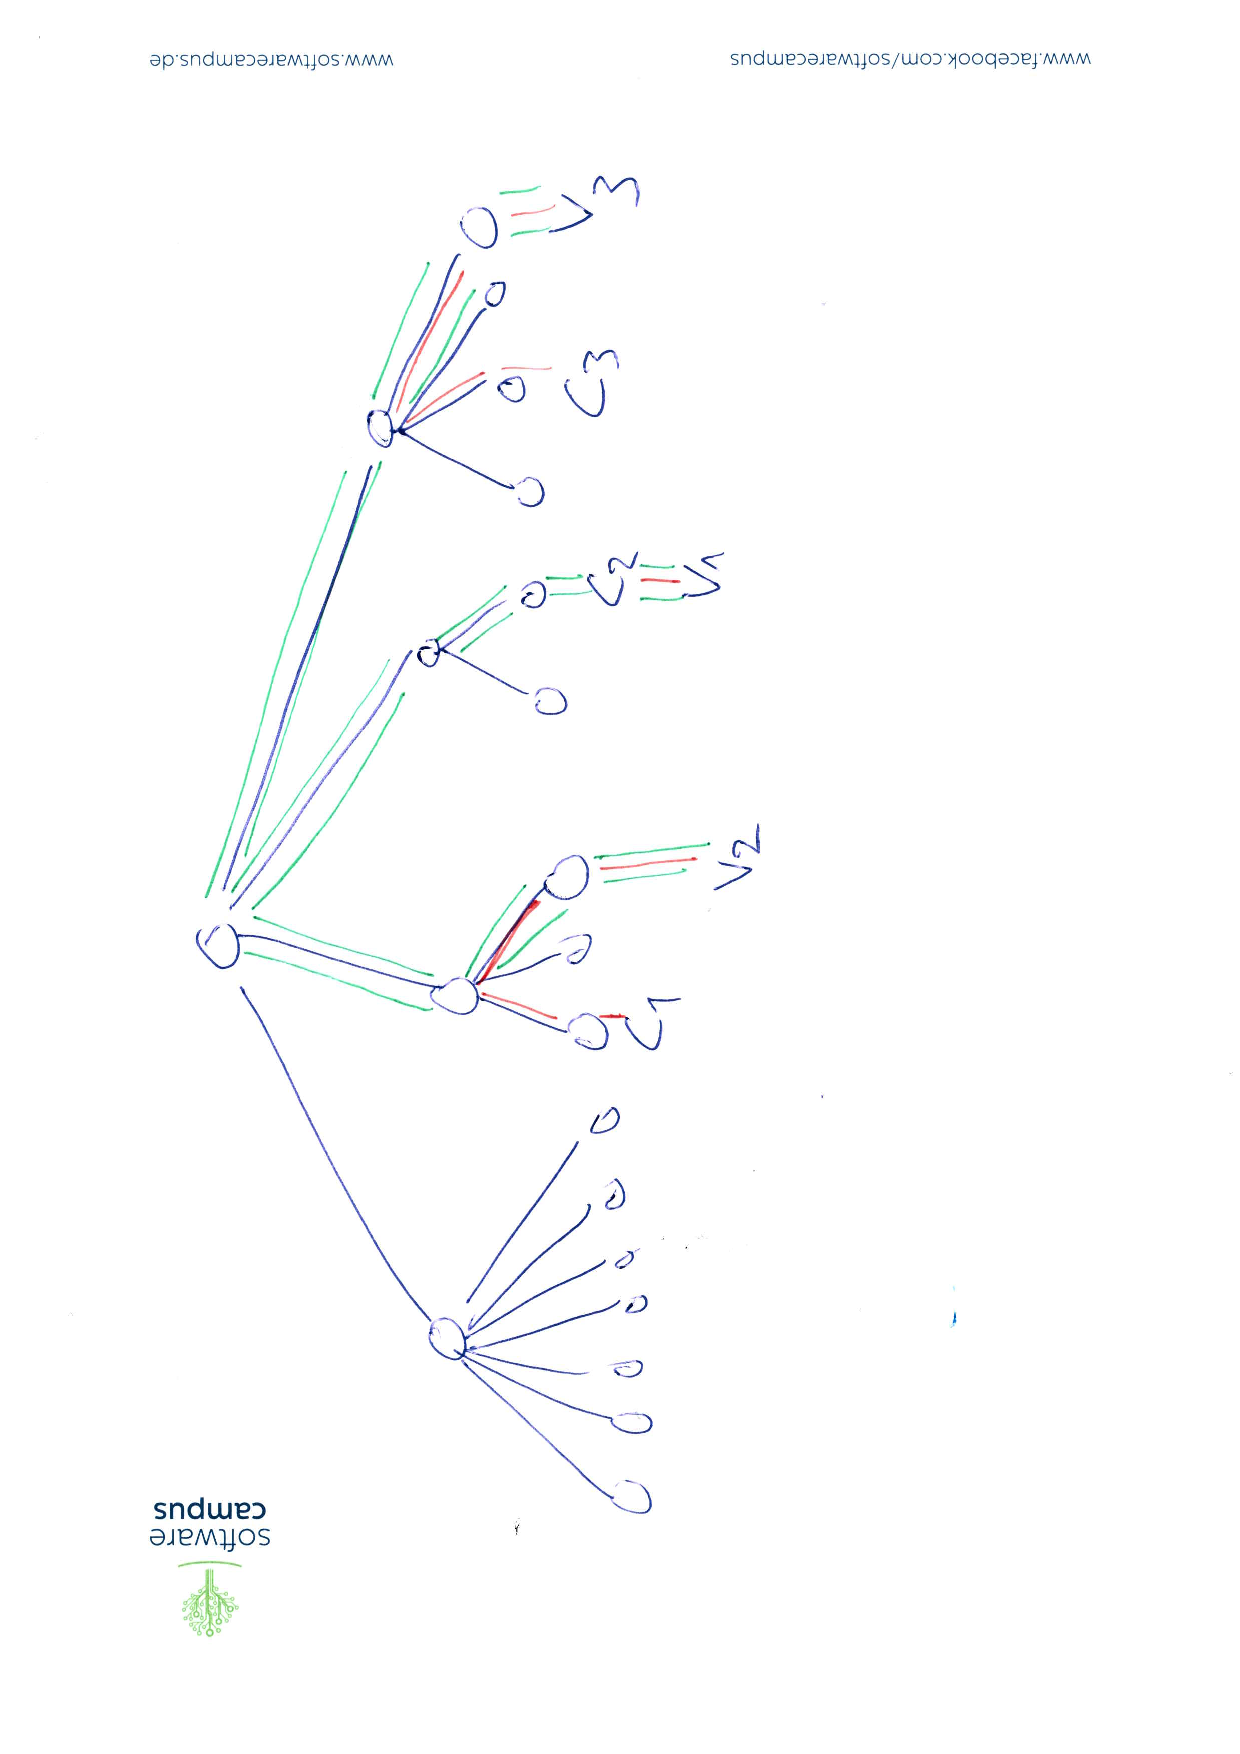
\includegraphics[angle=270,origin=c, height=7cm]{figs/model_fig_skteches/cv}
\caption{solution for problem with cv}
\end{figure}

%So
%far our model accounted bandwidth which is consumed to transfer data from it's
%location in the physical topology to the $\VM$ which will process it. However,
%due to the nature of distributed jobs, the $\VM s$ will also comunicate with
%each other. While we denoted the costs of transfering a chunk over a (1-hop)
%link with $b_t$, we will refer to the bandwidth costs of transfering data
%between a pair of $\VM s$ with $b_c$.


\subsection{Redundant Chunks - $r$}

This property specifies that, instead of having a single chunk $\Chunk_j$, we
have $\RedundancyFactor$ redundant copies of each chunk
$\Chunk_{j_1},\dots,\Chunk_{j_\RedundancyFactor}  \in \Chunks$. These copies are
entirely equal, and only one instance of a specific chunk type (e.g.
$\Chunk_{j_2}$) has to be read by one VM $\VirtualNode_j \in \VirtualNodes$.
Note that we assume chunks to be atomic - they cannot be read from two different
locations, requiering only $\CostTrans / 2$  bandwidth.

\begin{figure}

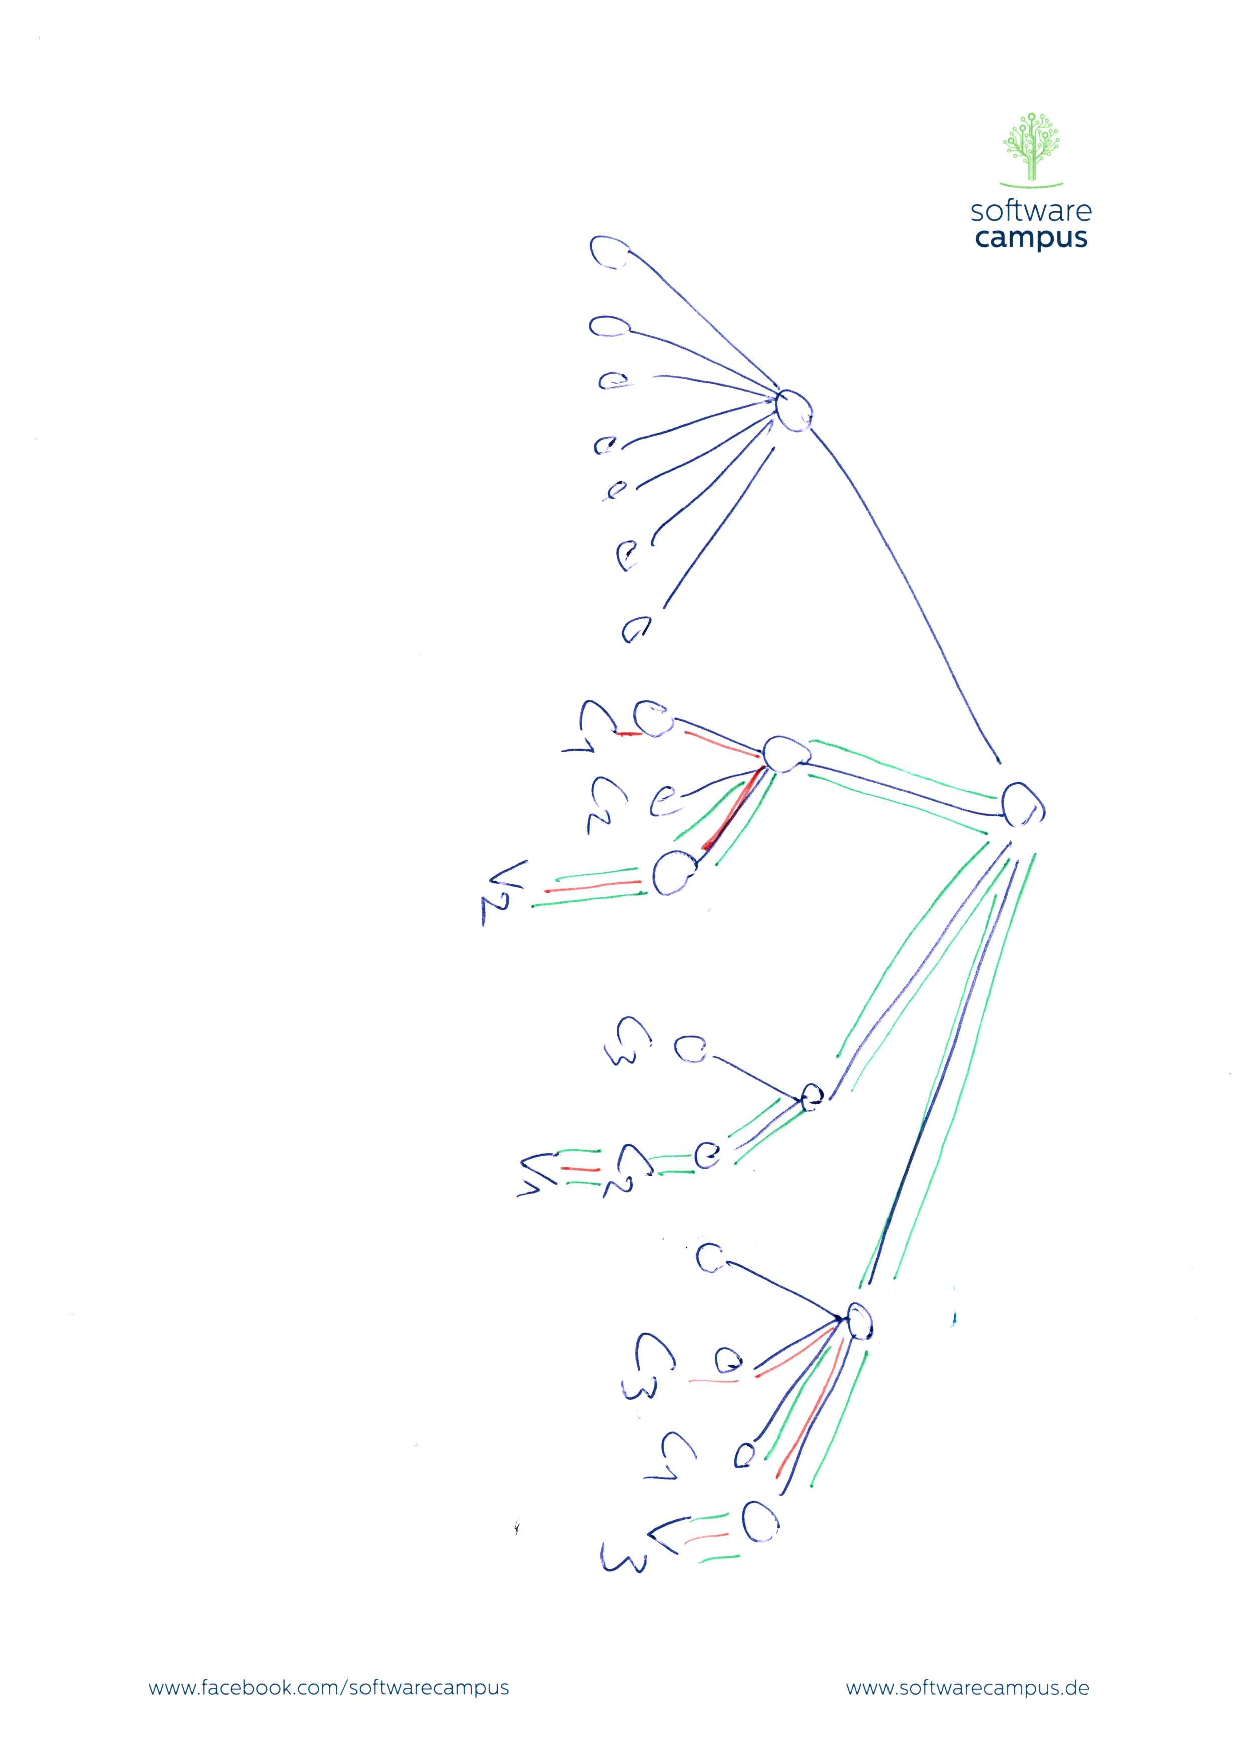
\includegraphics[angle=90,origin=c, height=7cm]{figs/model_fig_skteches/r_cv}
\caption{solution for problem with r}
\end{figure}




\subsection{Multiple Chunks per VM - $ma$}

This extension increases the processing capacities of the VMs. Instead of the
basic 1:1 ratio of VMs and chunks, this extension allows a VM to have $\MaFactor
\in \mathbb{N}^+$ many $\VmSlots$, which can all process chunks. We assume,
that the data which has to
be transferred to the VM from the chunks cannot be aggregated, and $\Vms =
\ChunkTypes / \MaFactor$.

\begin{figure}

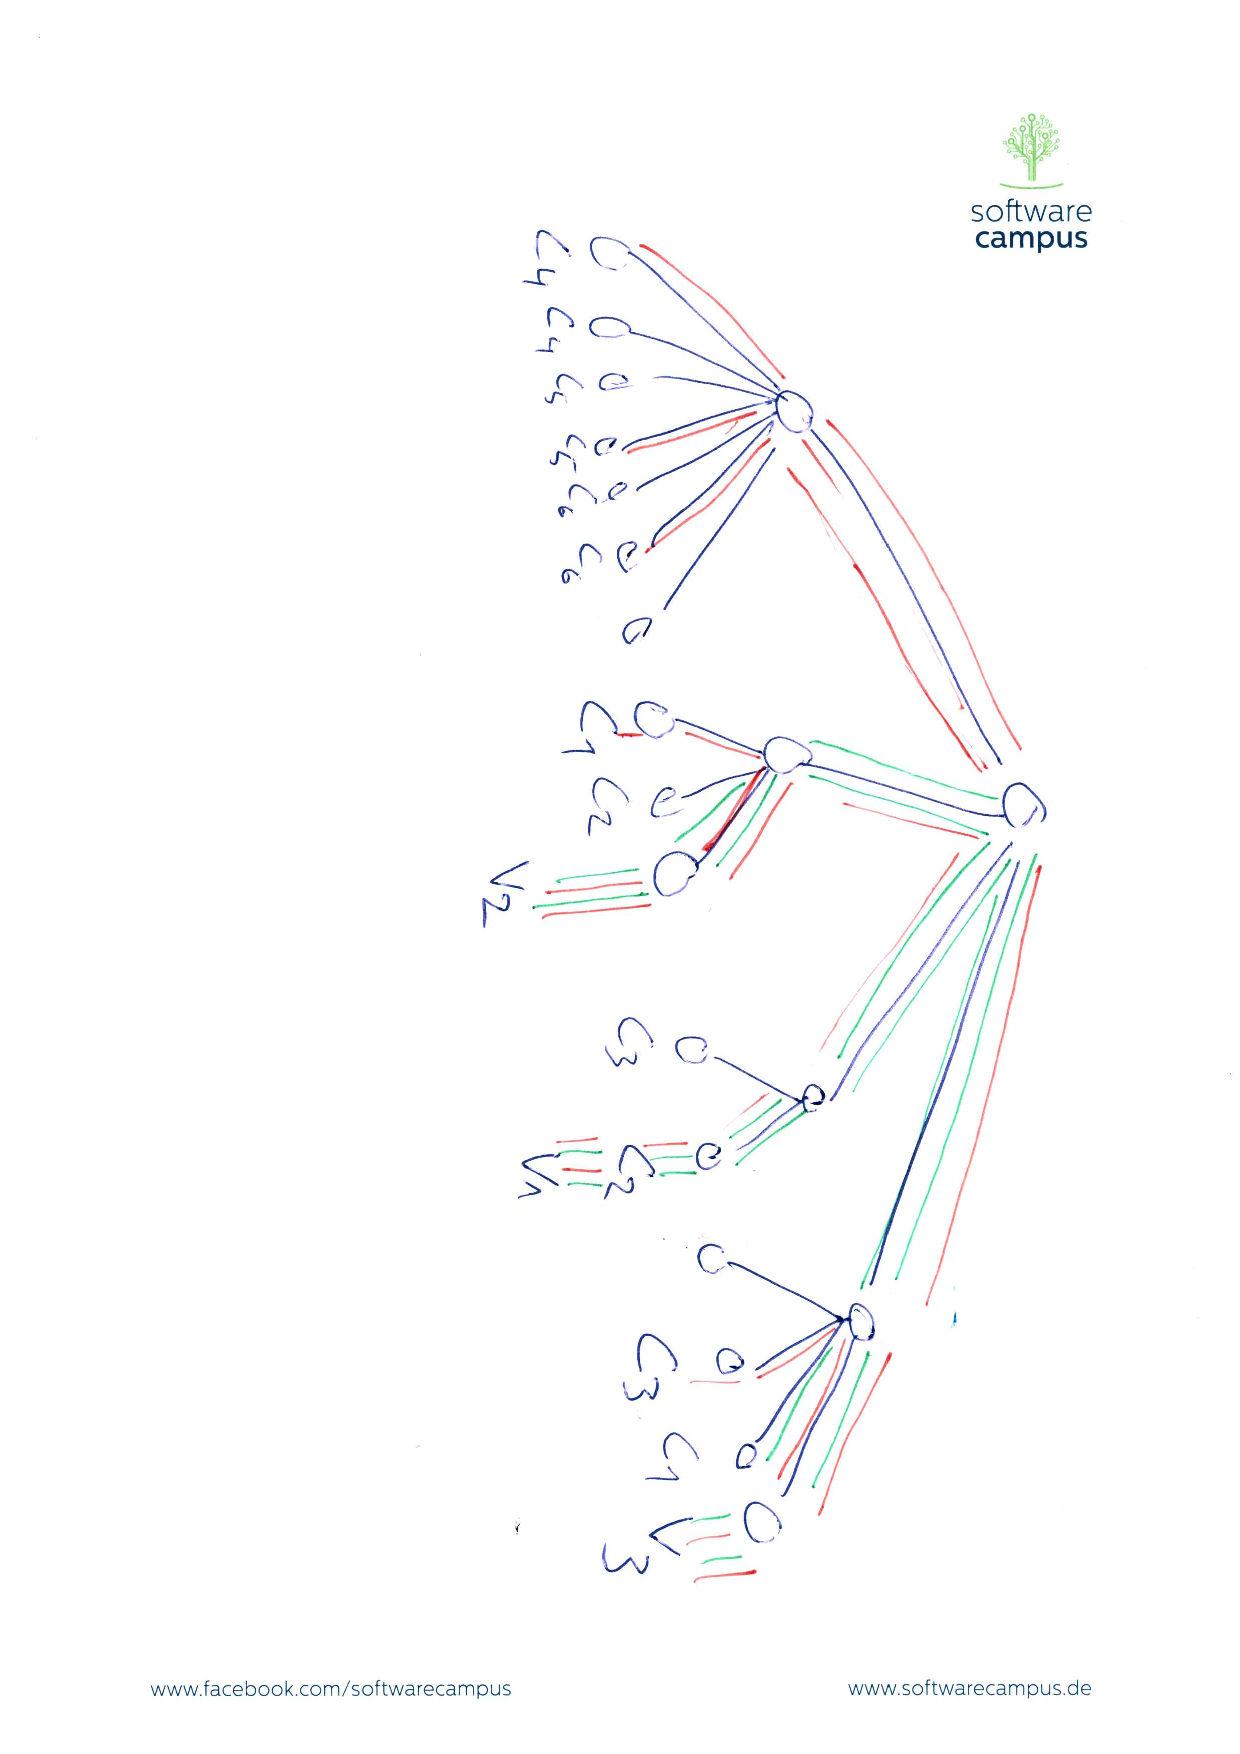
\includegraphics[angle=90,origin=c, height=7cm]{figs/model_fig_skteches/ma_r_cv}
\caption{soltion with ma}
\end{figure}

\subsection{Bandwidth Constraints - $bw$}

So far we only focussed on computing minimal bandwidth costs. However, in
reality the bandwidth which a single link can offer is limited. This model
extension limits the available bandwidth on each link $\SubstrateEdge_i \in
\SubstrateEdges$ in the host graph $\Tree$. We denote the capacity limitations
by $\Capacity : \SubstrateEdges \rightarrow \mathbb{R}$. The sum of all
bandwidth costs on this link, may never exeed it's capacity. Be aware that
this extension introduces infeasible instances.

\begin{figure}

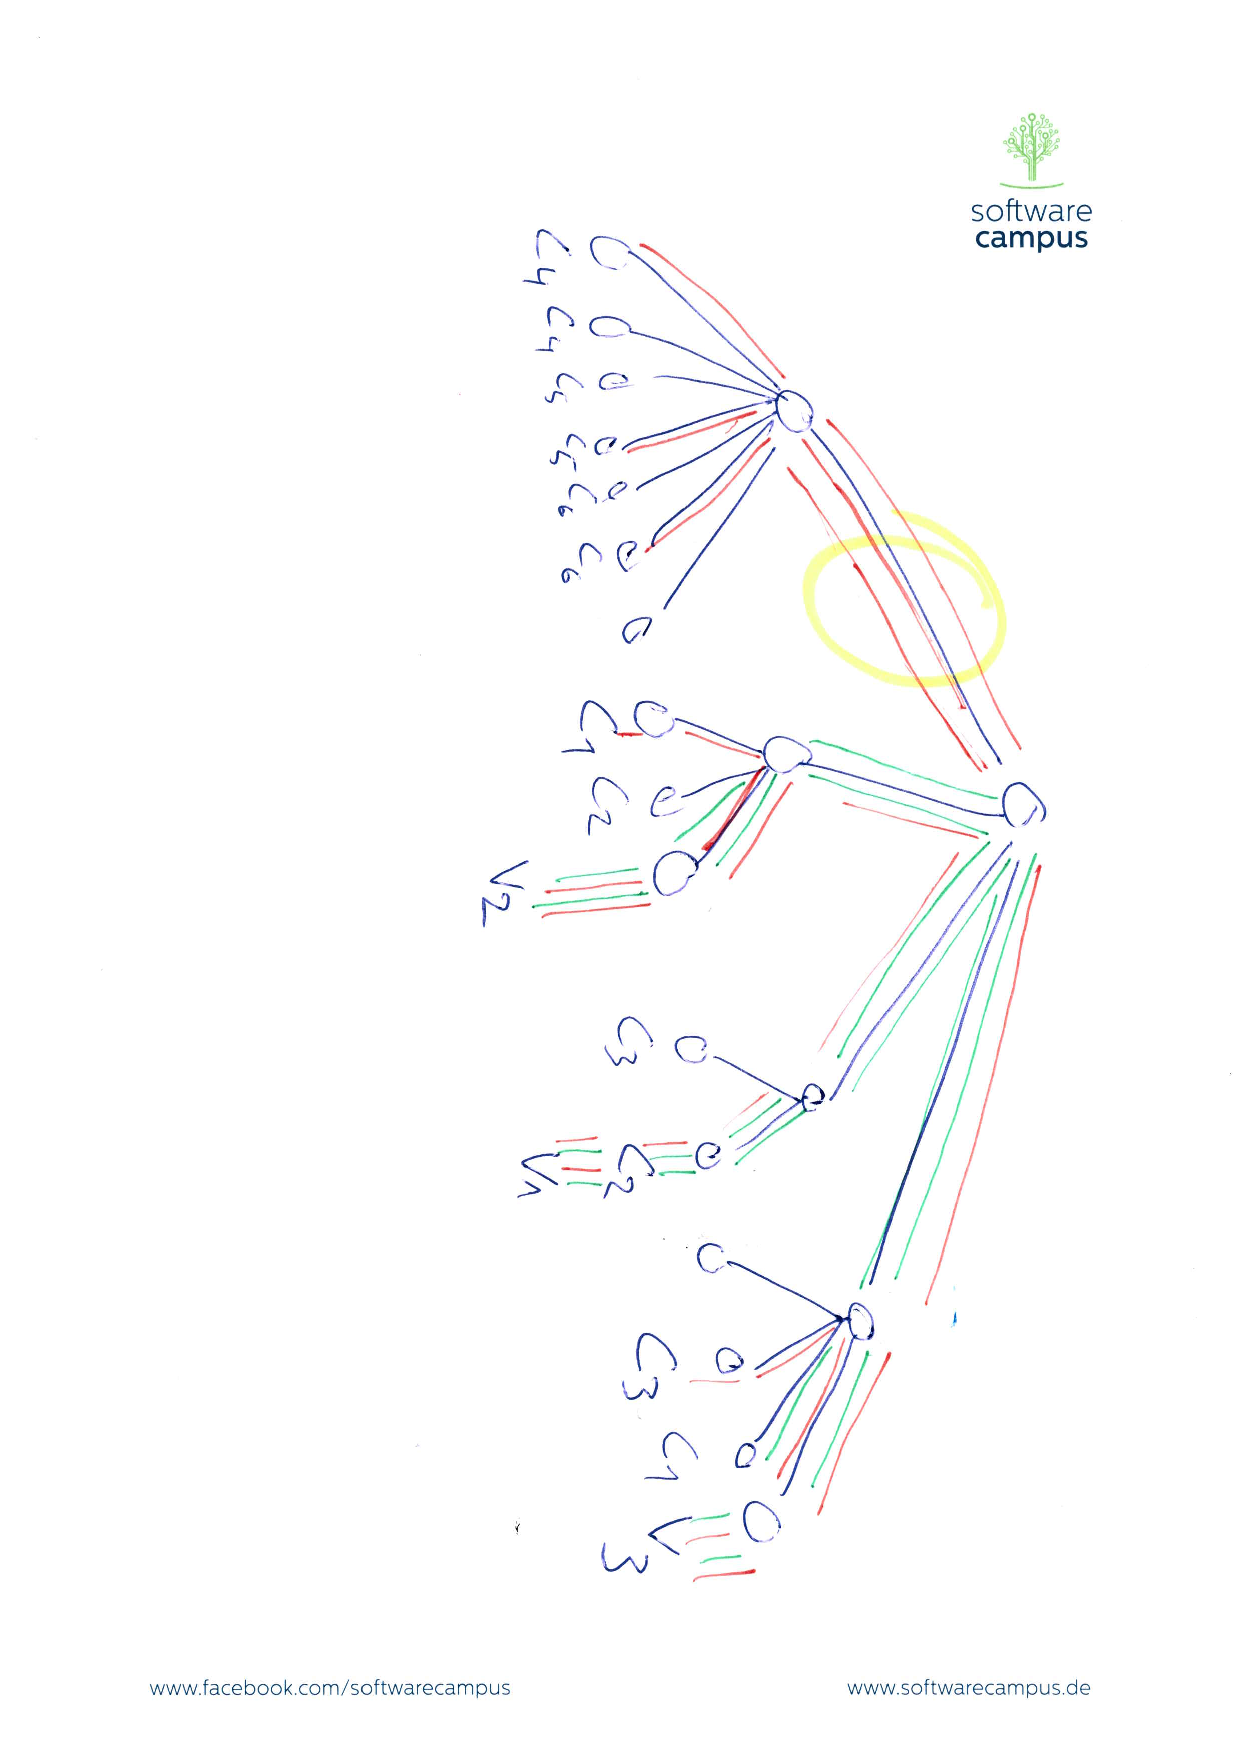
\includegraphics[angle=90,origin=c, height=7cm]{figs/model_fig_skteches/bw_ma_r_cv}
\caption{The bandwidth exceeds the capacity - independent of the chosen assignment}
\end{figure}
\subsection{Free VM Placement - $fp$}

The Free VM Placement property describes a variant of our simple model, where
the positions of the VMs are not given in the problem statement but are
rather chosen by the described strategy. Concretely, $\NodeMapping$ is no
longer given, but part of the optimization within $\Problem$. We assume that
each leaf can only host one VM.

\subsection{Combined models} In this paper we analyse combinations of the
different properties listed above.

\begin{figure}[htbp]
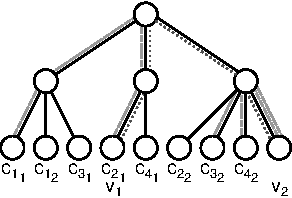
\includegraphics[width =\columnwidth]{figs/model_ma_r_cv}
\caption{An example instance of $\Problem$ with $ma$ + $cv$ + $r$. An
optimal solution is indicated by the dashed (transport costs) and dotted
(communication costs) lines. }
\label{fig:model_combined}
\end{figure}

An example of this can be seen in Figure~\ref{fig:model_combined}, which shows
an instance of $\Problem$, with the additional properties $ma$, $cv$ and $r$.
The host graph consists of 14 nodes. 9 nodes are leaves; 2 VMs are allready
embedded on leaves; with $\RedundancyFactor = 2$ and $\MaFactor = 2$ we have 4
chunk types, and two VMs of each type. The solution to this instance is also
depicted: The data from $\Chunk_{1_1}$ and $\Chunk_{2_1}$ is read by
$\VirtualNode_1$, $\Chunk_{3_2}$ and $\Chunk_{4_2}$ are read by
$\VirtualNode_2$. The dashed light gray lines indicate transport
costs $\CostTrans$. Note that no bandwidth is neccessary to transport data from
$\Chunk_{2_1}$ to $\VirtualNode_1$, since these are collocated. The link
connecting the node, which hosts $\VirtualNode_2$ with it's parent, the
transport costs ammount to $2 \CostTrans$ - indicated by two dashed lines. In
addition to this, the figure illustrates the communication costs $\CostCom$,
which are indicated by the dotted dark gray line.

%\subsection{Summary of our results}

\begin{figure}[htbp]
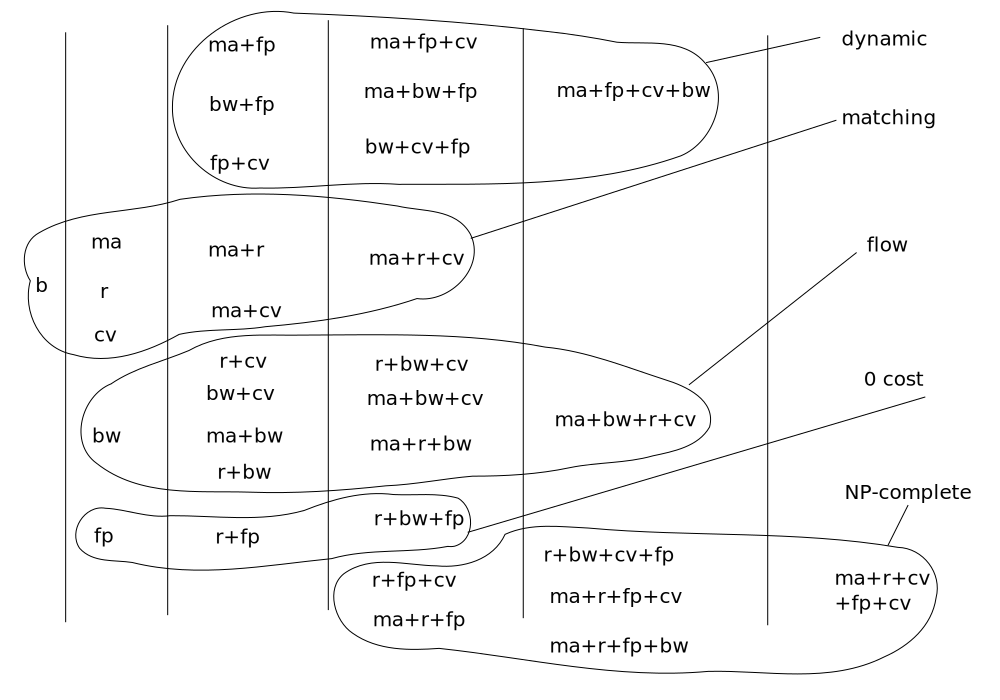
\includegraphics[width = \columnwidth]{figs/summary}
\caption{foo}
\label{fig:summary}
\end{figure}

This paper presents polynomial time algorithms or NP-hardness prooves for
\textit{all} possible comibnations of properties. An overview, of which problem
can be solved by which algorihms can be found in Figure~\ref{fig:summary}.

\begin{comment}
\begin{enumerate}
\item basic problem - M
\item ma - M
\item r - M
\item cv - reduces to basic problem
\item bw - F
\item fp - solution of 0 cost
\item ma + r - M
\item  ma + bw - F
\item ma + cv - reduces to ma
\item ma + fp - D
\item r + bw - F
\item r + cv - reduces to r
\item r + fp - solution of 0 cost
\item bw + cv - reduces to bw
\item bw + fp - D
\item fp + cv - D
\item ma + r + bw - F
\item ma + r + cv - reduces to ma + r
\item ma + r + fp - N
\item ma + bw + cv - reduces to ma + bw
\item ma + bw + fp - D
\item ma + fp + cv - D
\item r + bw + cv - reduces to r + bw
\item r + cv + fp - N
\item r + bw + fp - solution of 0 cost
\item bw + cv + fp - D
\item ma + r + bw + cv - reduces to ma + r + bw
\item ma + r + bw + fp - N
\item ma + r + cv + fp - N
\item ma + fp + cv + bw - D
\item r + bw + cv + fp - N
\item ma + r + bw + cv + fp - N
\end{enumerate}
\end{comment}

\end{appendix}


\end{document}
